\chapter{Tau Lepton Decay Modes Classification}
\label{chap:Tau}

\chapterquote{Give a man a fish and you feed him for a day; teach a man to fish and you feed him for a lifetime.}%
{}%: Blackwood's Magazine May 1830

The tau lepton has been studied extensively in the past at the Large Electron Positron Collider (LEP)\cite{Schael:2005am}. The tau lepton spin state, which can be derived from kinematic properties of tau decay products, can be used to measure the CP (the product of charge conjugation and parity symmetries) of the Higgs, via \HiggsToTauTau channel\cite{Berge:2015nua}. The tau pair polarisation correlation from a boson decay can be used to determine statistically if the parent boson is a  scalar or a vector, i.e. to differentiate \PH boson from \PZ boson.

 %The polarisation correlation of the tau pairs can be used to infer the spin of the parent boson, differentiating \HiggsToTauTau from \ZToTauTau.

\begin{comment}
\FIGURE{fig:tauTheorySpin} shows an example of  difference in distributions for the two channels.
\begin{figure}[!htbp]
\centering
% \begin{center}/\end{center} takes some additional vertical space
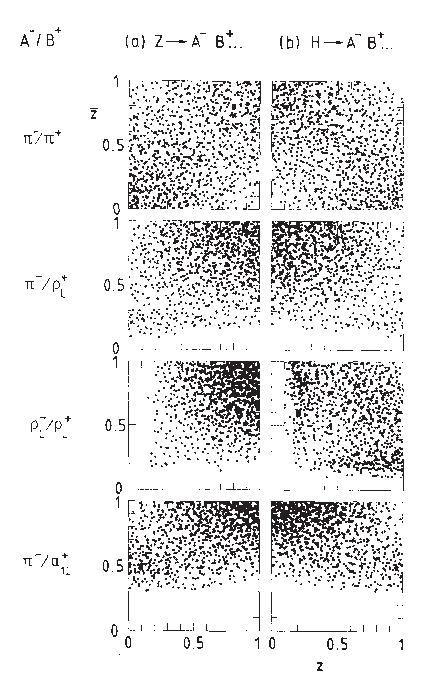
\includegraphics[width=.45\textwidth]{tau/theory}
\caption[An example of  difference in distributions for \HiggsToTauTau and \ZToTauTau.]
{
The two-dimensional distribution of (a) \HepProcess{\PZ \to \APtauon \Ptauon \to A^- B^+ \Pnut \APnut } (b) \HepProcess{\PHiggs \to \APtauon \Ptauon \to A^- B^+ \Pnut \APnut } events shown as functions of the energy fractions of $z = E_{A} / E_{\Ptauon}$ and $\overline{z} =  E_{B} / E_{\APtauon}$. In descending order the four sets of plots are for the (\APtauon, \Ptauon) pair decaying into (\Ppiminus, \Ppiplus), (\Ppiminus, $\rho_L^+$), ($\rho_L^-$, $\rho_L^+$) and finally (\Ppiminus, $a_{1L}^+$), each together with a \Pnut \APnut neutrino-pair. Plot is taken from \cite{Bullock:1991my}.
}
\label{fig:tauTheorySpin}
\end{figure}
\end{comment}

The efficiency of reconstructing tau decay modes can be also used as a benchmark for detector performance. Since tau lepton has a very short mean lifetime of 290\,fs \cite{Abreu:1991jn}, only tau decay products can be detected with the tracking detectors and calorimeters. Therefore, the performances of the calorimetric and track systems determine the ability to reconstruct the tau lepton decay products and identify different tau decay modes.

The main challenge in the tau lepton decay modes  classification is to reconstruct and to separate spatially close photons. At a centre-of-mass energy above tens of GeV, decay products of the tau lepton are often boosted.  Hence the EM showers from photons pairs from \Ppizero decay often overlap each other in the calorimeters.  Reconstructing the photon pair as separate entities requires good photon reconstruction algorithms. Hence the developed photon reconstruction algorithms described in \Chapter{chap:Photon} are used in this study.

% and a fine \ECAL spatial resolution
%Since the main difference in the topologies between some final states, for example \decayRhoFinalState and \decayAiPhoton final states,  is the number of photons from \Ppizero in the final state, the ability to reconstruct the photon pairs from \Ppizero as separate particles is crucial to differentiate tau decay modes.




%Many final states of the tau decay involves \Ppizero, where \HepProcess{\Ppizero \to \Pphoton \Pphoton}. 

%This chapter is organised as follows. Firstly, the choice of samples for the analysis will be discussed. The tau decay modes of interests are identified. The pre-selection cuts and variables used in the MVA classification are then discussed. The performance of the tau decay mode classification will be given, followed by an \ECAL optimisation study using the developed tau decay mode classification. Lastly, the  tau decay mode classification is further used in a proof-of-principle analysis to demonstrate the ability to identify Higgs boson from \PZ  boson using the tau pair decay channel.

%
%The impact of the \ECAL transverse spatial resolution on the tau decay classification is demonstrated as well.



\section{Overview of the analysis}

The analysis starts with defining the samples in \Section{sec:tauDecayModes}. Seven major tau lepton decay modes are chosen for the tau decay mode classification. The simulation and reconstruction of these tau lepton decays are described in \Section{sec:tauSim}.  Pre-selection of the events, discussed in \Section{sec:tauPreSel}, are such that events affected by the reconstruction and detector effects, which do not vary with the \ECAL cell sizes, are taken out of this analysis. After defining discriminative variables used in the MVA classification in \Section{sec:tauVar}, the classification is performed with a multivariate classifier. Since the decay products of a tau need to be classified into one of the seven decay modes, a multiclass classification, presented in \Section{sec:tauMVA}, is used to allow simultaneous classification between  multiple decay modes. Afterwards, the performance of the classification is described in \Section{sec:tauClassificationEff}.

The classification of the tau lepton decay modes are then  repeated for different energies of tau lepton decay to access the impact of the tau energy on the classification. The classification is also used to study the impact of the \ECAL cell sizes on the classification performance,  discussed in \Section{sec:tauECAL}. The classification is then utilised to demonstrate the ability to separate Higgs boson from \PZ  boson using the tau pair decay channel in a proof-of-principle analysis, described in the \Section{sec:tauHZ}.

% The difference in the spin of the boson reflects in the different spin correlation of the tau pair. By extracting the spin correlation, parent bosons can be separated.
%This classification is repeated for different energies of tau lepton decay to access the impact of energy on classification. The impact of the \ECAL design is studied afterwards, where the \ECAL square cell size is varied. An overall tau hadronic decay classification efficiency is constructed to allow direct and easy comparison between different detector design and different energies of the tau decay.

% The study of the tau final state classification in the context for the  \ECAL optimisation allows the analysis to discard reconstruction and detector issue that do not vary with the \ECAL design. For example, the early photon conversion that happens in the tracking detector would complicate the event topology. But since it is affected by the tracker design, it can be ignored in this analysis. \SECTION{sec:tauSim}  and \Section{sec:tauPreSel} discuss the pre-selection cuts to choose the signal samples and events for this analysis.

%The classification is performed with a multivariate classifier. Discriminating variables are calculated before feeding into the classifier.  A multiclass classicisation is used to allow simultaneous classification between  multiple final states, described in \Section{}.


%A proof-of-principle analysis to demonstrate the ability to identify \PHiggs from \PZ using  tau pair decay channel is presented in the \Section{}. The difference in the spin of the boson reflects in the different spin correlation of the tau pair. By extracting the spin correlation, parent bosons can be separated.

%The follow sections on the analysis use the a 50\,GeV tau lepton decaying sample, reconstructed with nominal the \ILD detector model.

\section{Event generation}
\label{sec:tauDecayModes}

%\section{Select single tau decay}  in a \ee collider for an electron-positron collider 
The studied tau lepton decay channel is \eeToTauTau, with a centre-of-mass energy of 100\,GeV.  To study the predominant effect of the tau lepton decays, decay modes with branching ratio above 2\% are classified. This results in seven tau lepton decay modes studied, which cover 92.58\,\% of the tau decay. The seven tau decay mode, their branching ratios, and detectable final states are  shown in \Table{tab:TauDecayMode}.


%Thrust axis is useful to separate each jet in a back-to-back two-jet event.
%Thrust value, $T$, is 1 for a perfect pencillike back-to-back two-jet event, and 0.5 for a perfect spherical event. The thrust value is useful in picking out back-to-back two-jet event.


%\subsection{Tau lepton decay modes}

%Tau lepton decays into a number of final states. 
% The most difficult final states to separate are \decayRhoFinalStateShort and \decayAiPhotonFinalStateShort, where photons from boosted \Ppizero are very challenging to reconstruct correctly.

\begin{table}[htbp]\centering
\smallskip
\begin{tabular}{l l r}
\hline
\hline
Decay modes & Detectable final states & Branching ratio\\
\hline
\decayElectron   &  \decayElectronShort  & $17.83{\pm0.04\%}$   \\
\decayMuon &	\decayMuonShort & $17.41{\pm0.04\%}$  \\
\decayPion  &   \decayPionShort	& $10.83{\pm0.06\%}$   \\
\decayRho   & \decayRhoFinalStateShort& $25.52{\pm0.09\%}$ \\
\decayAi   & \decayAiPhotonFinalStateShort	& $9.30{\pm0.11\%}$    \\
\decayAi  &	\decayAiPionFinalStateShort    & $8.99{\pm0.06\%}$  \\
\decayThreePionPhoton  &	\decayThreePionPhotonShort    & $2.70{\pm0.08\%}$  \\
\hline
\hline
\end{tabular}
\caption[Decay modes, detectable final state particles and branching ratios of the seven major \Pgtm decays.]
{Decay modes, detectable final state particles and branching ratios of the seven major \Pgtm decays. Values are taken from \cite{Agashe:2014kda}. \Pgtp decays similarly to \Pgtm.}
\label{tab:TauDecayMode}
\end{table}


\section{Simulation and reconstruction}
\label{sec:tauSim}


Two million \eeToTauTau events are simulated and reconstructed using the \ILD detector model. The beam specific effects that are not affected by the varying \ECAL cell sizes are not simulated, such as the initial state radiation and the beam induced background. An event display of \eeToTauTau interaction is shown in \Figure{fig:tauEvtDsp}. 


%As the study is aimed for optimisation study of the \ECAL cell sizes, t

\begin{figure}[tbph]
\centering
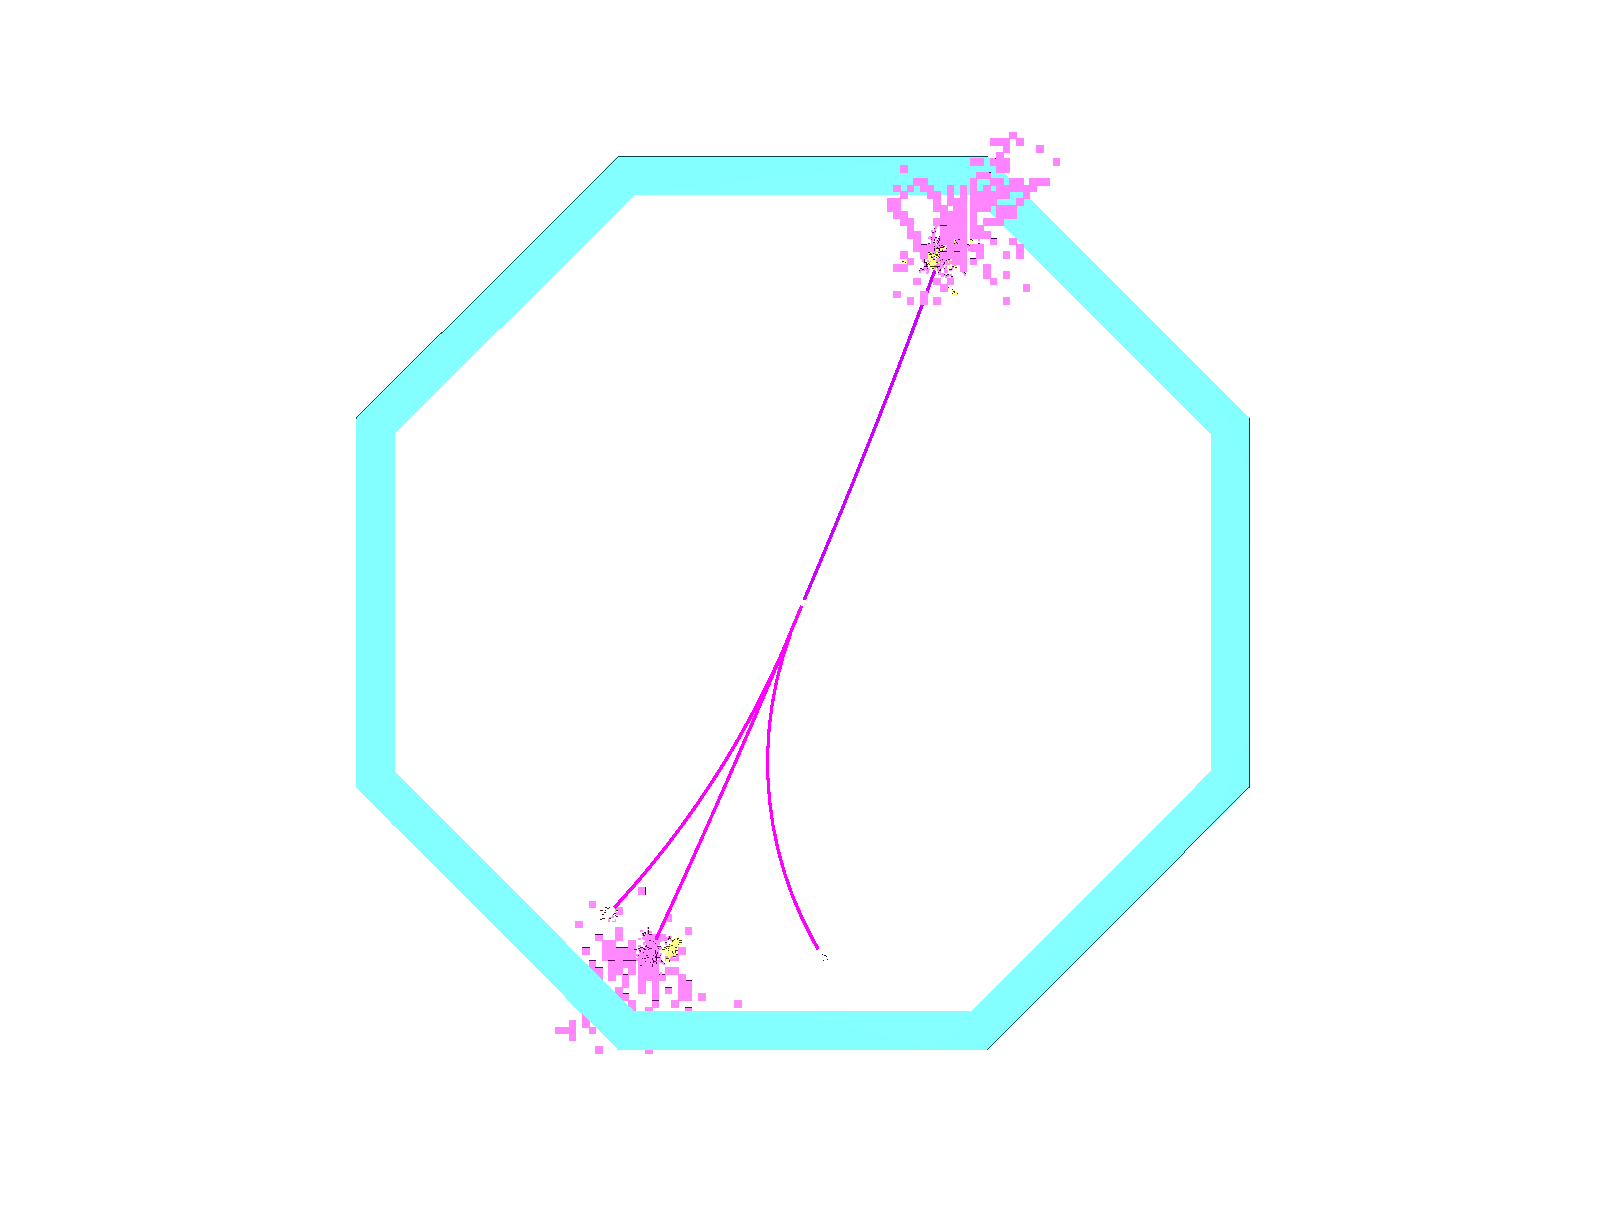
\includegraphics[width=0.65\textwidth]{tau/tau_evt_dsp2}
\caption{ An event display of a simulated \eeToTauTau event using the \ILD detector model. The top half of the event is a tau lepton decaying into \decayRhoFinalState final state and the bottom half of the event is a tau lepton decaying into  \decayThreePionPhoton final state. The purple lines are the tracks left by \Ppipm in the tracking detectors. The purple clusters are the calorimeter hits of \Ppipm in calorimeters. And the yellow clusters are the calorimeter hits of photon from \HepProcess{\Ppizero \to \Pphoton \Pphoton}. The blue region is the transverse cross section of the \ECAL barrel part along the beam line direction.}
\label{fig:tauEvtDsp}
\end{figure}



The software used for simulation and reconstruction is described in \Chapter{chap:Reconstruction}. Events are reconstructed with  \ilcsoft version v01-17-07 \cite{Gaede:82475} and \pandora version 3 \cite{Marshall:2015rfa}, where the photon reconstruction is discussed in \Chapter{chap:Photon}.


\section{Event pre-selection}
\label{sec:tauPreSel}

Pre-selection cuts select events using the truth information. Since the analysis is aimed for the optimisation of the \ECAL cell sizes, these pre-selection cuts are such that effects not affected by the changing of the \ECAL cell sizes are not considered in the analysis. These cuts allow the analysis to focus on the events with clear topologies. The pre-selection cuts are listed in \Table{tab:tauPreSel}. The fraction of events passing each pre-selection cut for individual decay mode are listed in \Table{tab:tauPreSelEff}.

One of the pre-selection cuts is to demand that the tau decay products  do not have photons converted to electron pairs in the tracking detector, determined with the truth information. These discarded events would have fewer photons and more electrons than expected in the final states, which changes the topologies of the final states. Shown in \Table{tab:tauPreSelEff}, only decay modes with photons in the final states are affected by this cut, as expected.


Another pre-selection cut requires the total energy of the non-neutrino tau decay products, $E_{vis,MC}$, to be greater than 5\,GeV, based on the truth information. If most energy of a tau lepton is carried by  neutrinos, non-neutrino decay products would have low energies and be difficult to be identified. Hence these events with low-energy non-neutrinos tau decay products are not used in the analysis. Decay modes with only one non-neutrino particle in the final states are mostly affected by this cut because more energies are carried by neutrinos, indicated in \Table{tab:tauPreSelEff}.

The last pre-selection cut is to discard events with tau decay products depositing energies in the gap region between barrel and the end cap part of the calorimeter. As the reconstruction   does not attempt to recover reconstruction in the gap region, there is a significant drop in the particle reconstruction efficiency in the gap region. The cut demands the absolute value of the polar angle of tau lepton, based on the truth information, $\absOf{\theta_{Z,MC}}$, is between 0.3 and 0.6\,rad to be contained in the end cap region, or is between 0.8 and 1.57\,rad to be contained in the barrel region. All decay modes are affected almost equally by this cut, suggested by numbers in \Table{tab:tauPreSelEff}.



%The no photon early conversion cuts only effective against final states with \Ppizero, as \Ppizero decays to a photon pair. For final states with one \Ppizero, about 77\% events survived. For final states with two \Ppizero, about 61\% events survived, which is roughly $0.77^2$. For the visible angle acceptance, final states with only one particle are affected the most, whilst final states with more than one particles typically have more visible energies. The polar angle acceptance efficiencies depend on the final states, as light final states are boosted and more likely in the forward region.



%An low visible energy event is discarded if the total energy of the tau lepton visible decay products is below 5\,GeV. Requirement of the tau decay in the barrel or the end cap part of the calorimeter is defined as the polar angle of the tau is $ 17.2\degree < |\theta_{Z}| < 34.4\degree$ or $ 45.8\degree < |\theta_{Z}| < 90\degree$.





The \eeToTauTau channel contains two tau leptons travelling in opposite directions. Since the tau decay mode classification is applied on a per tau lepton basis, the decay products of two taus in one event are divided into two collections for separate classification. Each collection of particles corresponds  to the decay products of one tau lepton.
The principle thrust axis vector is used to separation particles into two collections. Two collections are obtained based on the sign of the scalar product between the principle thrust axis vector  and the momentum vector of a particle. The principle thrust axis vector, $\hat{t}$, is chosen by maximising the classical event shape thrust \cite{PhysRevLett.39.1587}, $T$:
\begin{equation}
T = \max_{\hat{t}}\!\frac{\sum_{i}\absOf{\hat{t}\!\cdot\!\vec{p_{i}}}}{\sum_{i}\absOf{\vec{p_{i}}}}
\end{equation}
where $\vec{p_{i}}$ is the momentum vector of the particle $i$;   $\hat{t}$, is the unit principle thrust axis vector; and index $i$ is summed over all particles in an event. The principle thrust axis vector is the axis that most particle aligned to.


\section{Variables used in the MVA}
\label{sec:tauVar}


Having pre-selected events,  variables are carefully developed for the multivariate analysis (MVA). The full list of the variables are shown in \Table{tab:tauVaraibles}. The distributions of the four most powerful variables for selected tau decay modes are shown in \Figure{fig:tauVar}.

\subsection{\PFOs number variables}

The most crucial variables are the number of \PFOs of different types of particles. There are five \PFOs number variables used in MVA event selection: the number of charged particles (${N}_{\charge}$); the number of muons (${N}_{\Pmu}$); the number of electrons (${N}_{\Pe}$); the number of photons (${N}_{\Pgg}$); and the number of charged pions (${N}_{\Pgpm}$).

\FIGURE{fig:tauVarNCharge} shows the distributions of the number of charged particles for selected tau decay modes. Over 98\% one-prong final states have one track reconstructed, and around 95\%  three-prong final states have three tracks reconstructed. \FIGURE{fig:tauVarNPhoton} shows the distributions of the number of photons, which is powerful to distinguish final states with different numbers of \Ppizero s.

% and the overlap between \decayRhoShort and \decayAiPhotonShort is around 15\%. ${N}_{\Pgg}$ can also separate two 3-prong final states.
%${N}_{\Pmu}$, ${N}_{\Pe}$, ${N}_{\Pgpm}$ are useful to identify two leptonic final states, and further separate 3-prong final states from 1-prong final states.
%This is an excellent variable to separate 1-prong and 3-prong final states.  An orthogonal measurement is the number of reconstructed photons,  ${N}_{\Pgg}$, shown in \Figure{fig:tauVarNPhoton}.

\subsection{Invariant mass variables}

Five invariant mass variables participate the MVA classification: the invariant mass of all non-neutrino decay products ($m_{vis}$); the invariant mass of all charged particles ($m_{\charge}$); the invariant mass of all neutral particles ($m_{\neutral}$); the invariant mass of all photons ($m_{\Pgg}$); and the invariant mass of all charged pions ($m_{\Pgpm}$). \FIGURE{fig:tauVarMVis} shows the distributions of the invariant mass of all non-neutrino decay products for selected tau decay modes. Resonance structures can be seen for \Prho and \Pai decay modes in the figure.

%Invariant masses of different particles are good at characterising different final states. \FIGURE{fig:tauVarMVis} shows the invariant mass of the system. Clear reasonable peaks can be seen for \Prho and \Pai. The mass peak of  \decayAiPionFinalStateShort are much higher. $m_{\charge}$ and $m_{\neutral}$ are invariant masses of charged and neutral particles respectively. They separate final states with neutral particles from those without neutral particles. Similarly, $m_{\Pgg}$ and $m_{\Pgpm}$ identify final states with photons and with \Pgpm respectively.

\subsection{Energy variables}

Energy information helps to further separate different final states. Six energy variables are used in the MVA classification: the normalised total energy of all non-neutrino decay products ($\tilde{E}_{vis}$); the normalised total energy of the charged particles ($\tilde{E}_{\charge}$); the normalised total energy of the muons ($\tilde{E}_{\Pmu}$); the normalised total energy of the electrons ($\tilde{E}_{\Pe}$); the normalised total energy of the photons ($\tilde{E}_{\Pgg}$); and the normalised total energy of the charged pions ($\tilde{E}_{\Pgpm}$). All variables are normalised with respect to the energy of the associated tau lepton.

\subsection{Calorimetric information variables}


Two calorimetric information variable are used in the MVA classification: the fraction of the energy  deposited in the \ECAL over the  energy deposited in the calorimeters for all charge particles ($\% E_{\charge}$) and the fraction of the energy  deposited in the \ECAL over the  energy deposited in the calorimeters for all particles ($\% E$). These  two variables help to identify electrons and muons. For example, an electron deposits most energy in the \ECAL, and a muon deposits 5\% to 20\% energy in the \ECAL. The difference between two variables is that photons, which deposit most of their energy in the \ECAL, do not participate in the calculation of $\% E_{\charge}$.



\subsection{\texorpdfstring{\decayRhoShort and \decayAiPhotonShort} \, resonances reconstruction variables}
\label{sec:tauResonance}
\decayRhoShort and \decayAiPhotonShort decay modes are identified further using their invariant mass resonance structure. For example, \decayRhoShort decay mode contains a \Pgpm and a \Ppizero decaying into two photons. By selecting \Pgpm and photons consistent with \Prho mass, \decayRhoShort decay mode could be identified. The  \decayRhoShort decay mode hypothesis test is performed by minimising a  $\chi^{2}$ function:
\begin{equation}
\chi^{2} = {\left(\frac{m_{tot} -  m^{MC}_{\Prho}}{\sigma^{MC}_{\Prho}}\right)}^{2} + {\left(\frac{m_{\Pphoton \Pphoton} -  m^{MC}_{\Ppizero}}{\sigma^{MC}_{\Ppizero}}\right)}^{2} \,,
\label{eqn:tauRho}
\end{equation}
where $m_{\Pphoton \Pphoton}$ is the invariant mass of two photons; $m_{tot}$ is the invariant mass of the  two photons and one \Pgpm; $m^{MC}_{\Prho}$ and $m^{MC}_{\Ppizero}$ are true masses of \Prho and \Ppizero, respectively, taken from \cite{Agashe:2014kda}; and $\sigma^{MC}_{\Prho}$ and $m^{MC}_{\Ppizero}$ are the half width of the invariant mass distribution of reconstructed \Prho and \Ppizero, respectively, obtained using the truth information. All combinations of photons and \Pgpm are tested. Two variables obtained in this minimisation and used in the MVA classification are the invariant mass of the two photons in the fit, $m_{\Pgpz}\parenths{\rho}$, and  the invariant mass of the  two photons and one \Pgpm, $m_\rho$.


Similarly, \decayAiPhotonShort decay mode can be identified using an extended minimisation function:
\begin{equation}
\chi^{2} = {\left(\frac{m_{tot} -  m^{MC}_{\Pai}}{\sigma^{MC}_{\Pai}}\right)}^{2} + {\left(\frac{m_{\Pphoton1 \Pphoton2} -  m^{MC}_{\Ppizero}}{\sigma^{MC}_{\Ppizero}}\right)}^{2}  + {\left(\frac{m_{\Pphoton3 \Pphoton4} -  m^{MC}_{\Ppizero}}{\sigma^{MC}_{\Ppizero}}\right)}^{2} \,,
\end{equation}
where \Prho has been replace by \Pai and other variables are defined in the same way as in the previous $\chi^2$ function in \Equation{eqn:tauRho}. Two photon pairs and one \Pgpm are needed for this minimisation. Both photon pairs are required to be consistent with the \pionToPhoton. Three variables obtained in this minimisation and used in the MVA classification are the invariant mass of the first two photons in the fit, $m_{\Pgpz}\parenths{\Pai}$; the invariant mass of the last two photons in the fit, $m^*_{\Pgpz}\parenths{\Pai}$; and the invariant mass of the four photons and one \Pgpm, $m_{\Pai}$. The first photon pair is defined to have a invariant mass closer to the invariant mass of the \Ppizero than the second photon pair.  \FIGURE{fig:tauVarMA1} shows the distributions of the invariant mass of $m_{\Pai}$ under \decayAiPhotonShort hypothesis test for selected tau decay modes. Only the distribution for \decayAiPhotonShort decay mode has a resonance peak at \Pai mass.

%Comparing to simple invariant mass distribution in \Figure{fig:tauVarMVis}, \decayAiPhotonShort mass peak is enhanced.
%\decayAiPhotonShort reconstruction &  \multicolumn{1}{R{0.6\textwidth}}{  $m_{\Pgpz}\parenths{\Pai}$, $m^*_{\Pgpz}\parenths{\Pai}$, $m_{\Pai}$} \\

The $\chi^{2}$ functions for both hypothesis test are adapted for events where the event reconstruction fails to reconstruct enough photons. Relevant terms are dropped from the expression if there are fewer photons reconstructed  than required in the $\chi^{2}$ functions.

\subsection{Separate \decayElectronShort from \decayPionShort}

The Particle ID obtained from \pandora is used extensively to reconstruct variables used in the MVA classification. In particular \pandora uses a wide range of information to determine the electron ID. However, extra variables are used in this analysis to help further identifying electrons, which could be mistaken as \Pgpm by \pandora reconstruction.

An electron leaves a characteristic electromagnetic  (EM) shower in the \ECAL, whilst \Pgpm doesn't. Variables characterising the  EM shower helps to identify \Pem. Three variables are used in the MVA classification: the start layer of the longitudinal shower ($t_0$); the fractional difference between observed and expected longitudinal shower profile describing the longitudinal EM shower ($\delta{l}$); and $\langle{w}\rangle$, a measure of the EM shower transverse width. These variables are  taken from the photon ID step in the photon reconstruction in \pandora, described in \Section{sec:photonLikelihood}.

Another type of information to differentiate an EM shower from a early hadronic shower from a \Pgpm is the calorimeter hit information. Two variables used in the MVA classification are: the average energy of a calorimeter hit ($\bar{E}_{hit}$) and the average fraction of possible minimum ionising calorimeter hit for all particles ($\%MIP$)

Last information used to separate \Pem from \Pgpm is the track-momentum-calorimeter-energy consistency check. The variable used in the MVA classification is the calorimeter energy divided by the track momentum for all particles ($\Delta E/P$).

The variables used to separate \Pem from \Pgpm  are obtained via a modified version of \pandora.
%This variable is found to help to differentiate \decayElectronShort from \decayPionShort final state.


%EM shower profile & $\delta{l}$, $t_0$, $\langle{w}\rangle$ \\
%Calorimeter hit info. & $\bar{E}_{hit}$, $\%MIP$ \\
%Track info. & $\Delta E/P$ \\




\begin{figure}[htbp]
\centering
% \begin{center}/\end{center} takes some additional vertical space
\begin{subfigure}[b]{0.45\textwidth}
 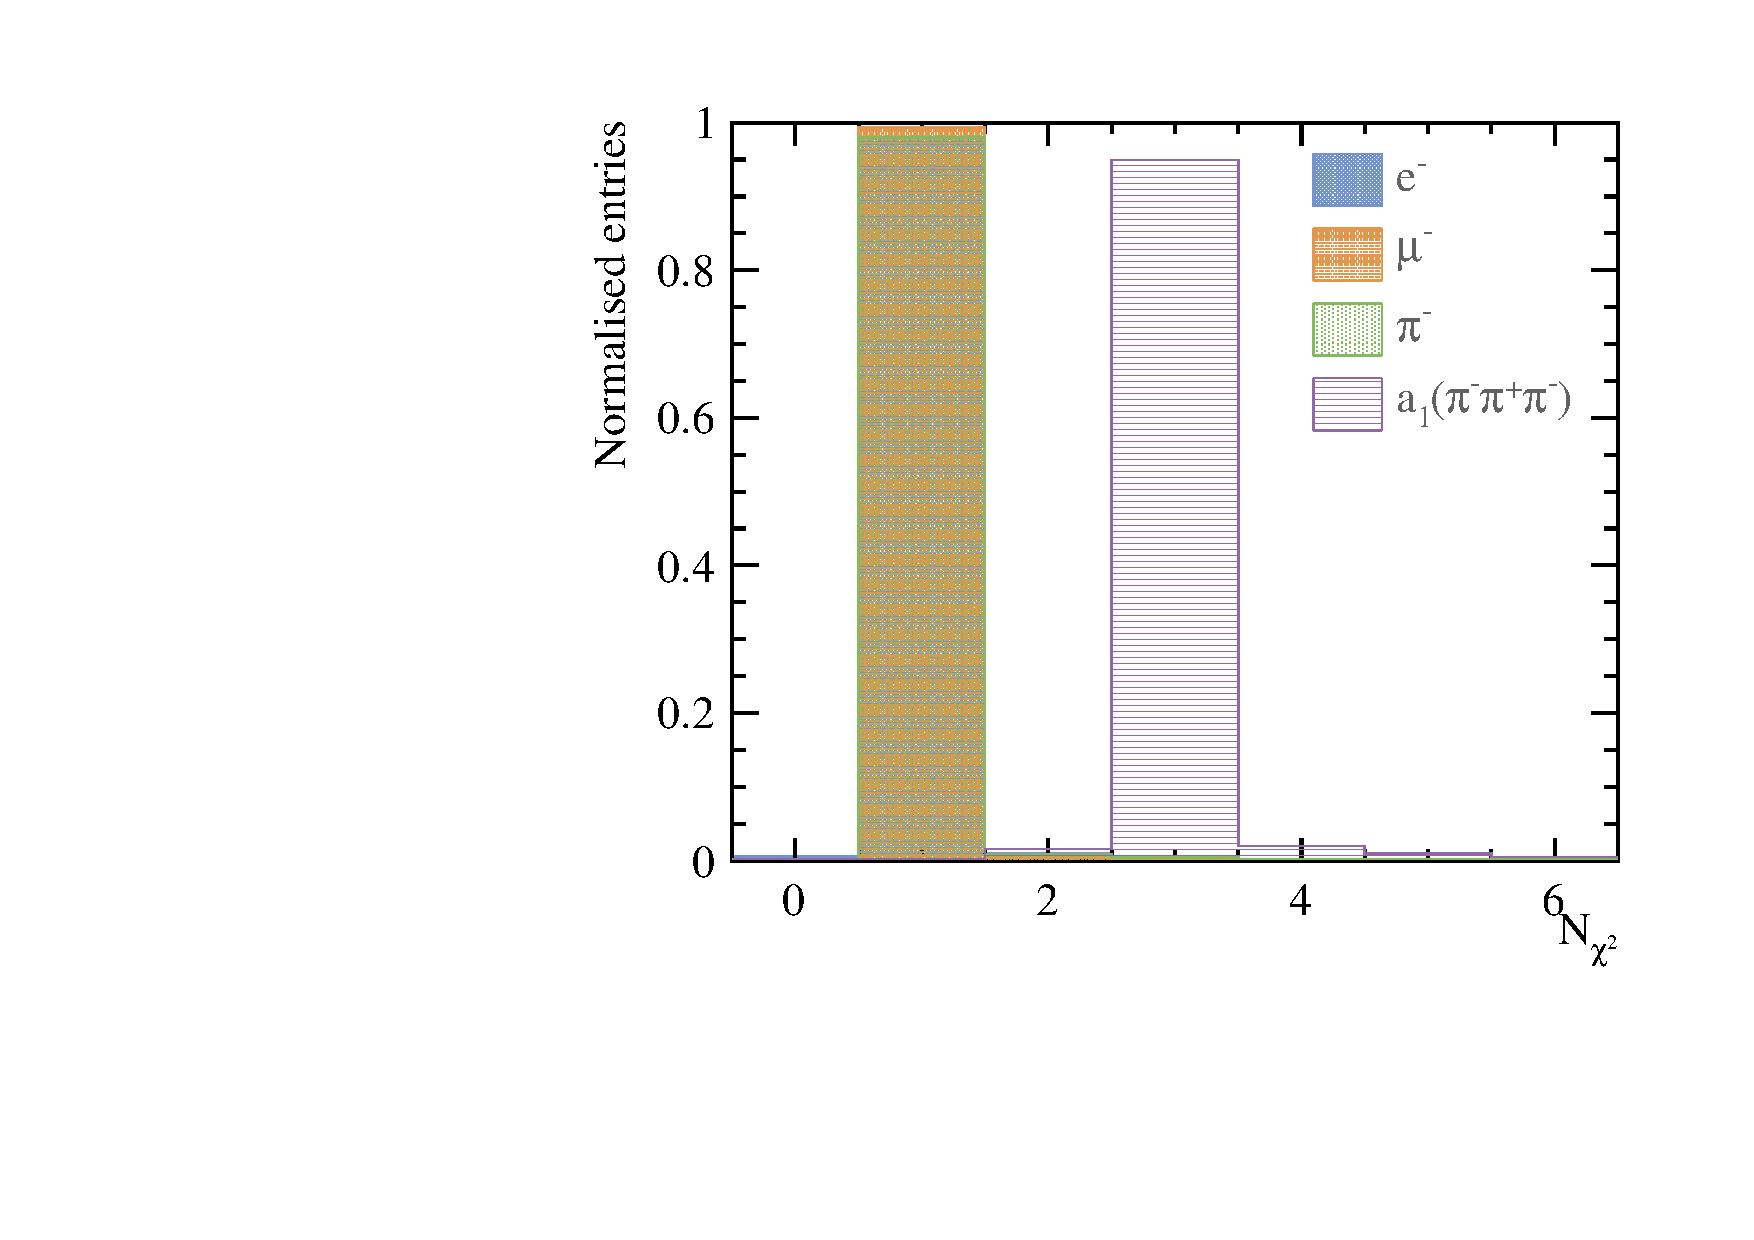
\includegraphics[width=\textwidth]{tau/var2/nCharge_100GeV_improved.pdf}
  \caption{}
  \label{fig:tauVarNCharge}
\end{subfigure}
\begin{subfigure}[b]{0.45\textwidth}
 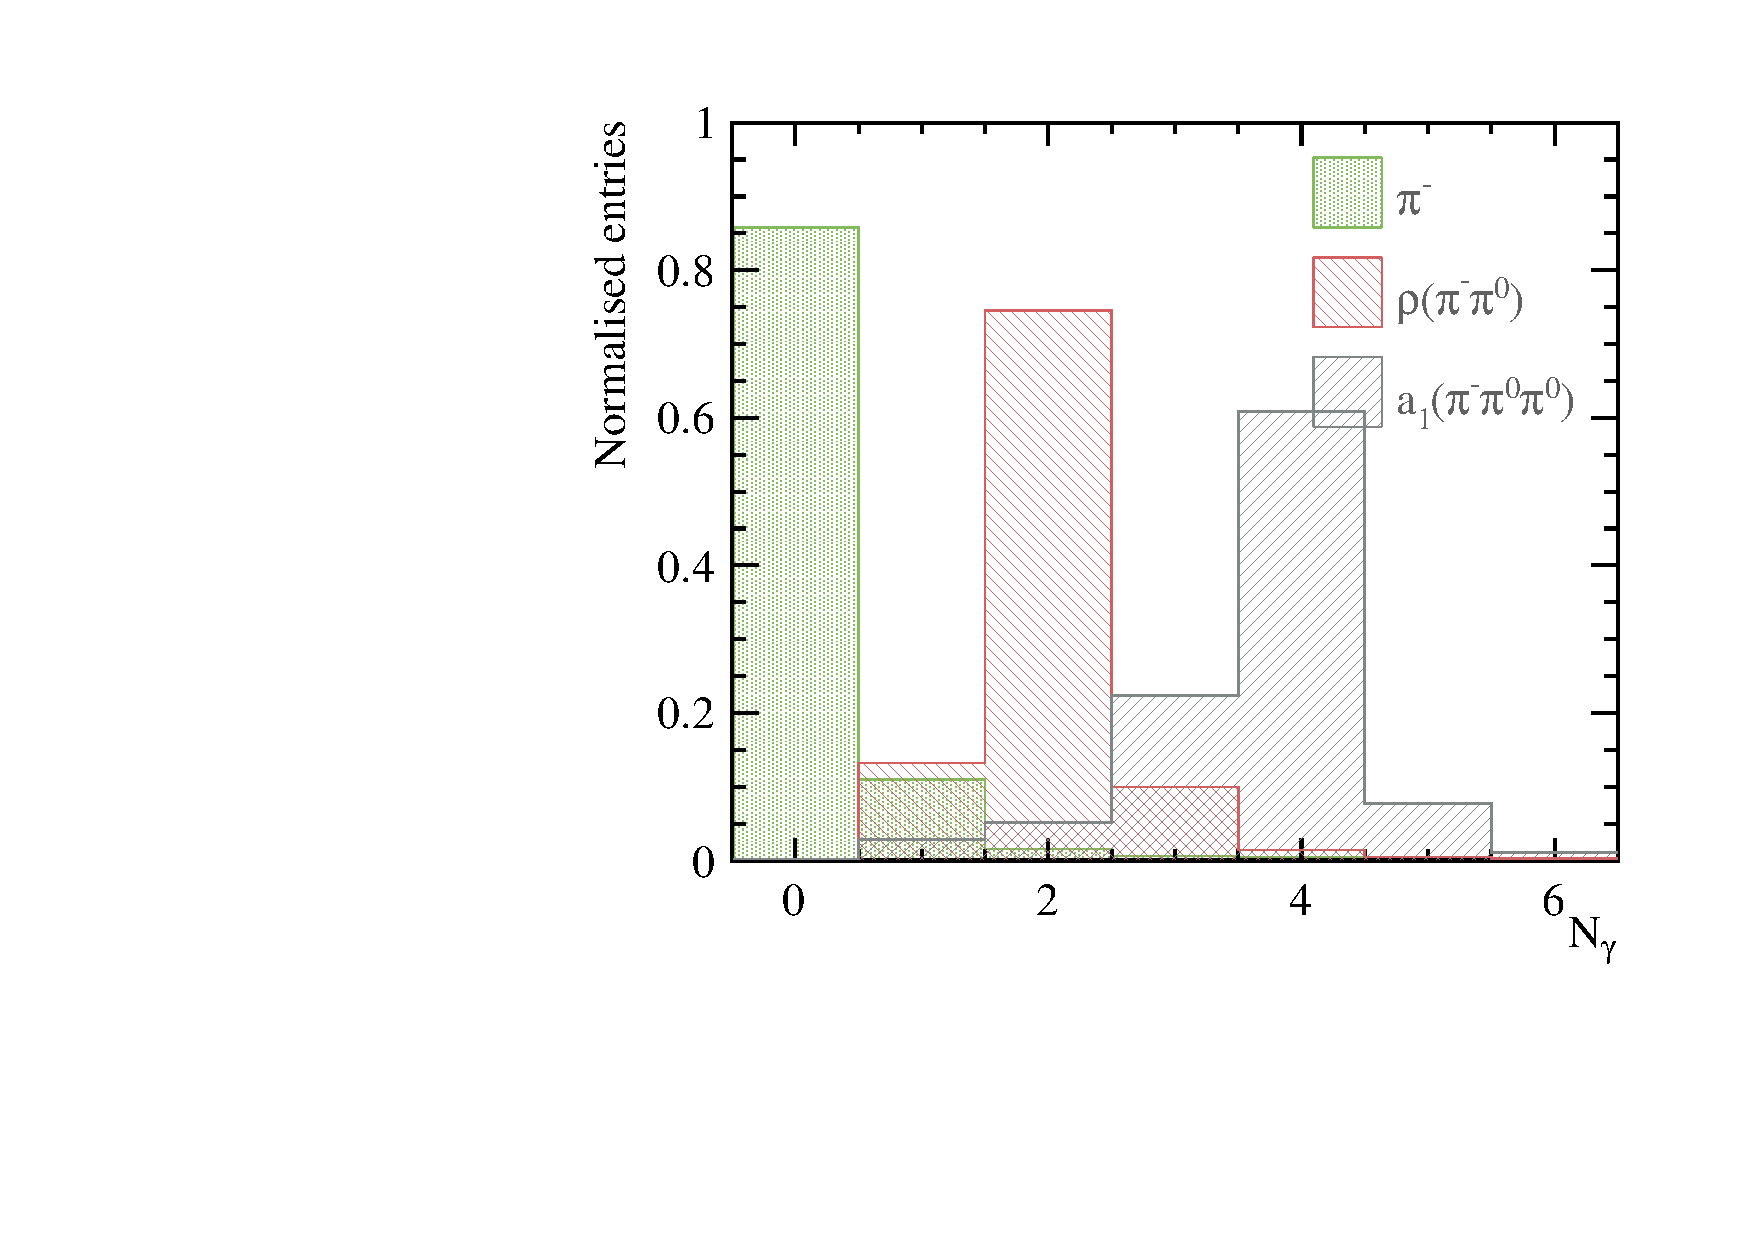
\includegraphics[width=\textwidth]{tau/var2/nPhoton_100GeV_improved.pdf}
  \caption{}
  \label{fig:tauVarNPhoton}
\end{subfigure}
\begin{subfigure}[b]{0.45\textwidth}
 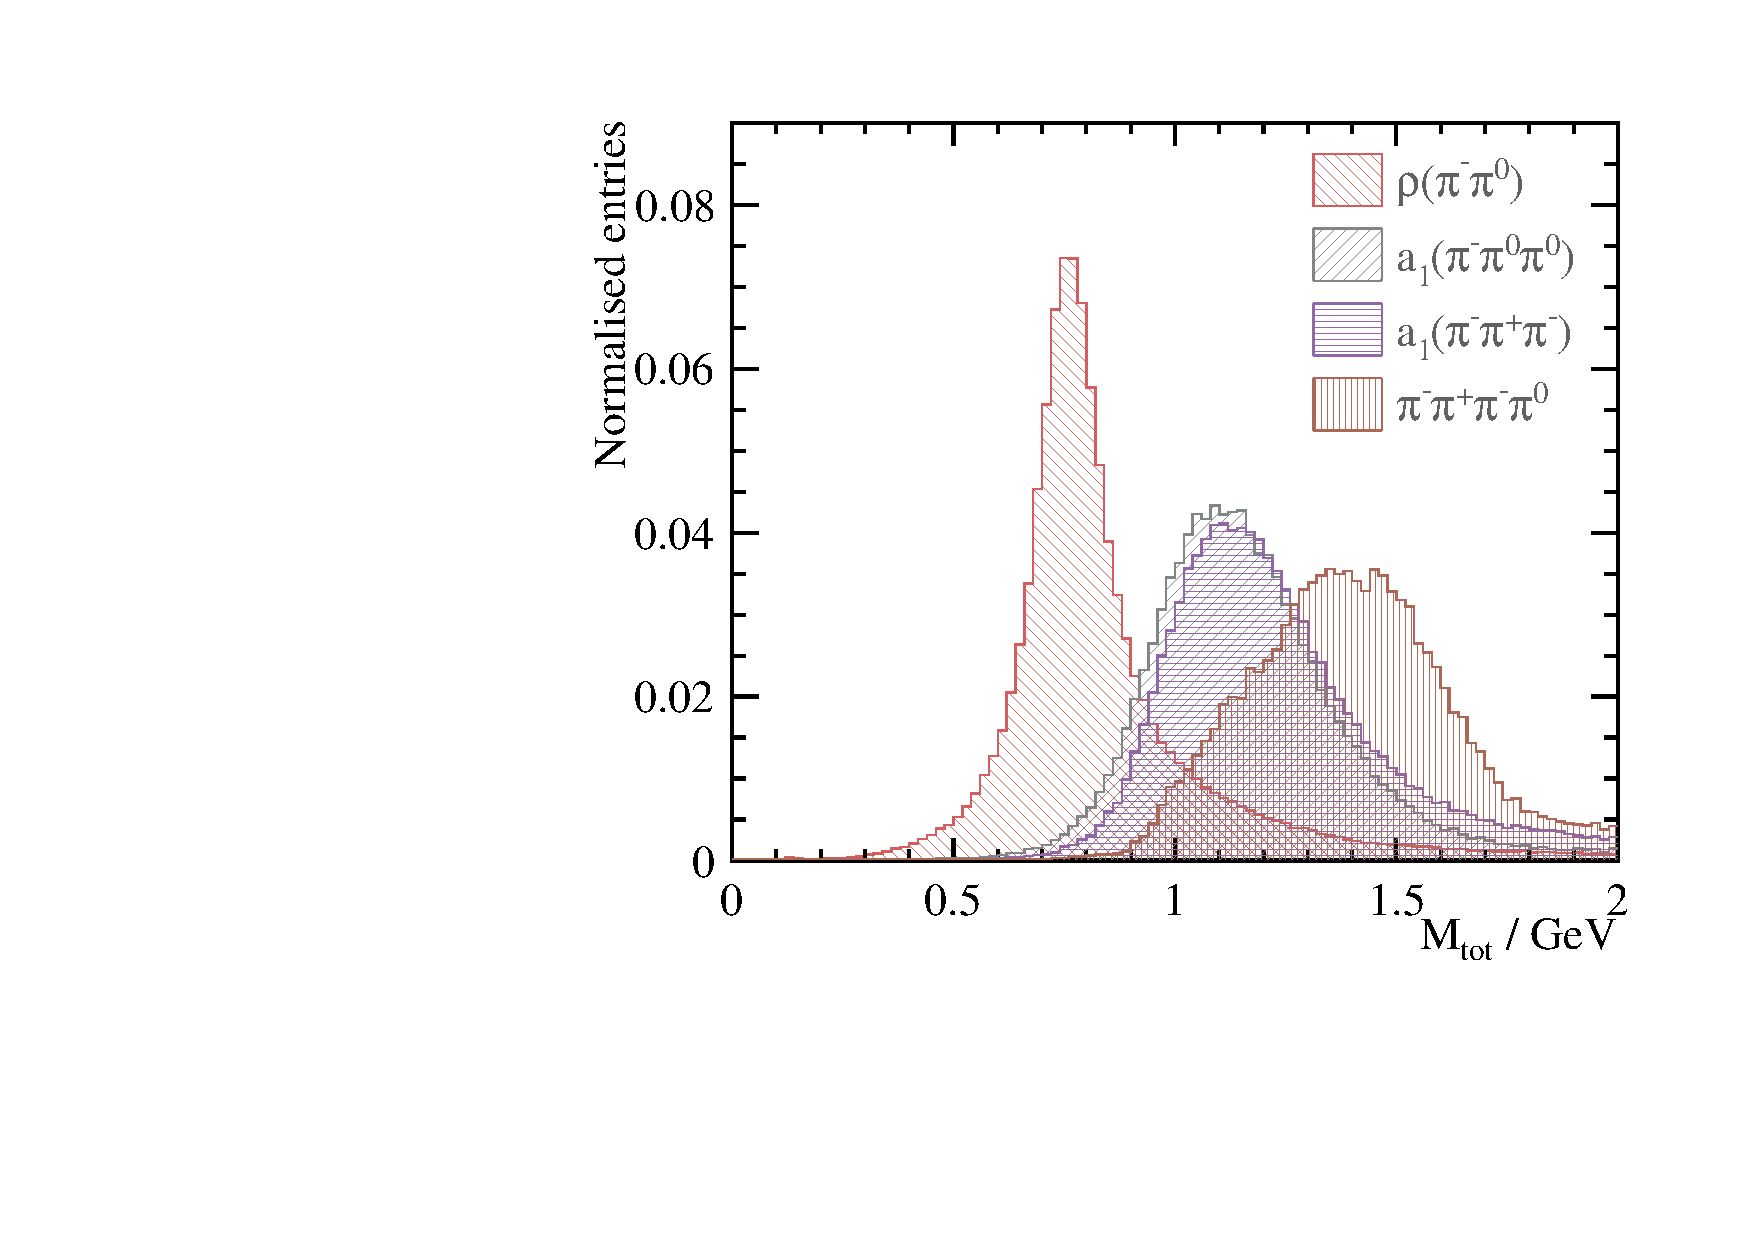
\includegraphics[width=\textwidth]{tau/var2/mVis_100GeV_improved_zoom.pdf}
  \caption{}
  \label{fig:tauVarMVis}
\end{subfigure}
\begin{subfigure}[b]{0.45\textwidth}
 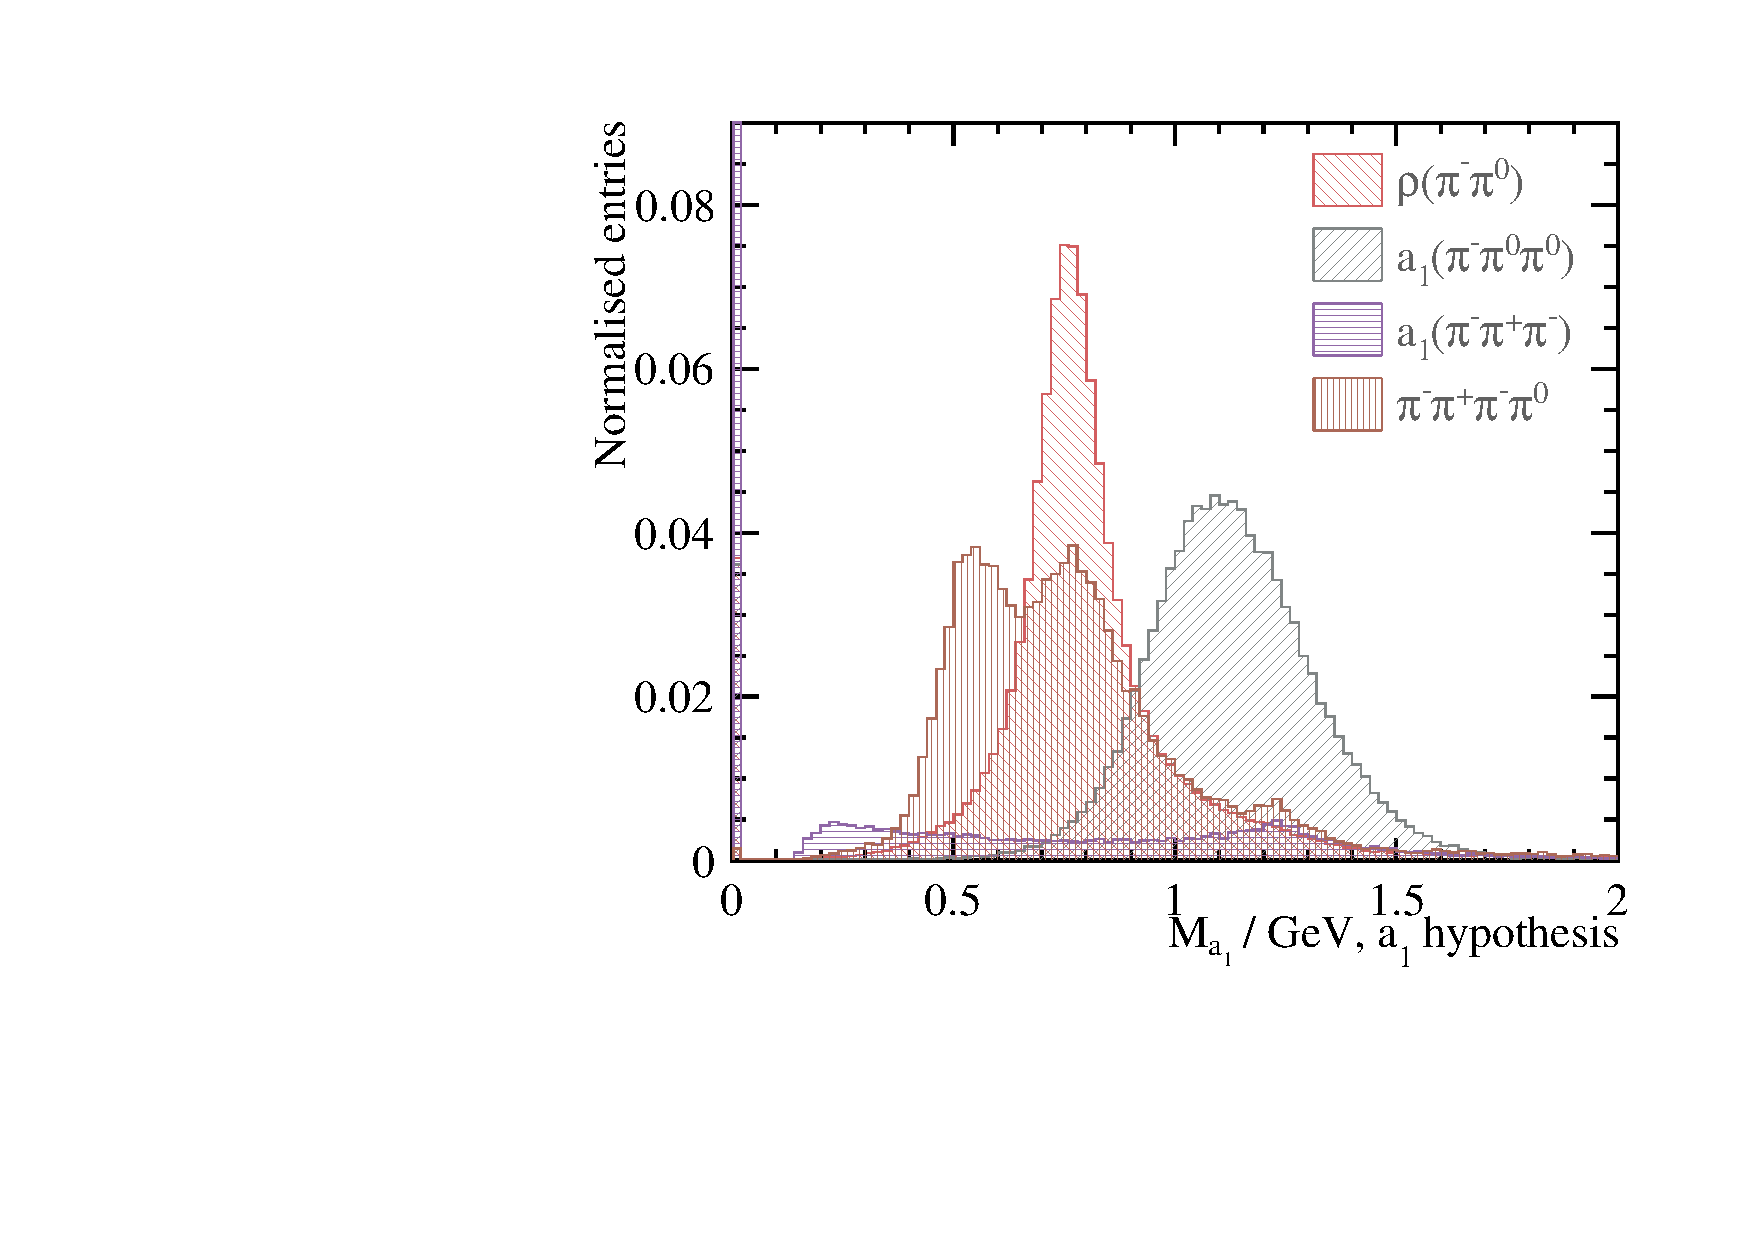
\includegraphics[width=\textwidth]{tau/var2/mA1A1Fit_100GeV_improved_zoom.pdf}
  \caption{}
  \label{fig:tauVarMA1}
\end{subfigure}

\caption
{Distribution for a) the number of charged particle (${N}_{\charge}$); b) the number of photons (${N}_{\Pgg}$); c) the invariant mass of all non-neutrino decay products ($m_{vis}$); and d) the invariant mass of the \Pai, reconstructed with \decayAiPhotonShort hypothesis. Area under the curve for each decay mode is normalised to 1. Decay modes in all plots are selected using the truth information.}
\label{fig:tauVar}
\end{figure}

\begin{table}[!htbp]\centering
\begin{tabular}{lr}
\hline
\hline
Category &  Variable \\
\hline
\PFOs number  & \multicolumn{1}{R{0.6\textwidth}}{  ${N}_{\charge}$, ${N}_{\Pmu}$, ${N}_{\Pe}$, ${N}_{\Pgg}$,  ${N}_{\Pgpm}$} \\
Invariant mass &  \multicolumn{1}{R{0.6\textwidth}}{$m_{vis}$, $m_{\charge}$, $m_{\neutral}$, $m_{\Pgg}$, $m_{\Pgpm}$} \\
Energy & \multicolumn{1}{R{0.6\textwidth}}{ $\tilde{E}_{vis}$,  $\tilde{E}_{\charge}$, $\tilde{E}_{\Pmu}$, $\tilde{E}_{\Pe}$, $\tilde{E}_{\Pgg}$,  $\tilde{E}_{\Pgpm}$} \\
Calorimetric info. &   \multicolumn{1}{R{0.6\textwidth}}{ $\% E_{\charge}$,  $\% E$ } \\
\decayRhoShort reconstruction & \multicolumn{1}{R{0.6\textwidth}}{  $m_{\Pgpz}\parenths{\rho}$, $m_\rho$} \\
\decayAiPhotonShort reconstruction &  \multicolumn{1}{R{0.6\textwidth}}{  $m_{\Pgpz}\parenths{\Pai}$, $m^*_{\Pgpz}\parenths{\Pai}$, $m_{\Pai}$} \\
EM shower profile & $\delta{l}$, $t_0$, $\langle{w}\rangle$ \\
Calorimeter hit info. & $\bar{E}_{hit}$, $\%MIP$ \\
Track info. & $\Delta E/P$ \\
\hline
\hline
\end{tabular}
\caption
{Variables used in the MVA classification for the tau lepton decay mode classification.}
\label{tab:tauVaraibles}
\end{table}

\section{Multivariate Analysis}
\label{sec:tauMVA}
For the multivariate analysis, the multiclass class of the TMVA package \cite{Therhaag:2009dp} was used to perform a multiclass classification, which classifies seven tau lepton decay final states simultaneously. The multiclass classifier is an extension of a standard two-class signal-background classifier. The discussion on multivariate analysis can be found in \Section{sec:pandoraMVA}. In particular, the multiclass classifier is discussed in \Section{sec:pandoraMVAmulticlass}.

The multiclass classifier used is Boosted Decision Tree with Gradient boost (BDTG). The optimisation of the BDTG classifier followed the strategy in \Section{sec:pandoraMVAoptimisation}. The optimised parameters are listed in \Table{tab:tauBDTparameters}. An explanation of the variables can be found in \Section{sec:pandoraMVAbdtVar}.  Half of the randomly selected samples were used in the training process and the other half were used for testing.

\begin{table}[!htbp]\centering
%\small
\begin{tabular}{lr}
\hline \hline
 Parameter &  Value \\
\hline
Depth of tree & 5 \\
Number of trees & 3000 \\
Boosting & gradient boost \\
learning rate of the gradient boost & 0.1 \\
metric for the optimal cuts & Gini Index \\
bagging fraction & 0.5 \\
Number of bins per variables & 100 \\
End node output & yes/no \\
\hline \hline
\end{tabular}

\caption
{Optimised parameters for the Boosted Decision Tree with Gradient boost multiclass classifier. See \Section{sec:pandoraMVAbdtVar} for a detailed explanation of variables.}
\label{tab:tauBDTparameters}
\end{table}


\section{Tau decay mode classification efficiency}
\label{sec:tauClassificationEff}
The classification efficiencies for the seven tau decay modes are shown in \Table{tab:TauSelExample}. Bold numbers show the correct classification probabilities.

%For example, 99.8\% events of true \decayElectronShort decay mode are reconstructed correctly.

For the \decayElectronShort decay mode,   99.8\%  correct classicisation efficiency is achieved. For \decayMuonShort decay mode,  99.5\% correct classicisation efficiency is achieved, due to an effective track reconstruction and muon reconstruction algorithms in \pandora.

For the \decayPionShort decay mode, 3.4\% events were misclassified as \decayRhoShortest decay events. If the reconstruction is unable to reconstruct the photon pair from \Ppizero decay in \decayRhoShortest decay mode, the \decayPionShort and \decayRhoShortest decay events would appear to  similar and misclassification is caused. On the other hand, only 0.9\% of \decayPionShort decay events are misclassified as \decayElectronShort decay, due to variables dedicated to separation between \Pem and \Ppiminus.

%The confusion with \decayElectronShort is at percent level, which is low due to the usage of EM shower variables. The percent level confusion with \decayAiPionShortest is because the tracking efficiency is at 98\%, where 2\% \decayPionShort events have more than one track reconstructed.

%confusion with \decayRhoShortest decay mode  is to due to differentiate two event topologies. Around 15\% of \decayPionShort events have at least one photon reconstructed, mostly due to the FSR.

For the \decayRhoShortest decay mode, most misclassification comes from the confusion with \decayAiPhotonShortest decay mode.  If the reconstruction is unable to resolve the all photon pair from \Ppizero decay in \decayRhoShortest and \decayAiPhotonShortest decay mode, the two decay modes would have similar topologies.

For the \decayAiPhotonShortest decay mode, the correct classification rate is the lowest among seven decay modes, as the \decayAiPhotonShortest decay final state is the most challenging to reconstruct correctly: two photon pairs and  one \Ppipm. The 9.5\% confusion with \decayRhoShortest is due to the same photon reconstruction failure issue. It should be noted that \Figure{fig:tauVarNPhoton} suggests that 30\% of \decayAiPhotonShortest events have fewer than four photons reconstructed, where the distribution overlaps with the distribution for \decayRhoShortest decay mode. The \decayAiPhotonShortest resonance reconstruction and the multiclass classifier reduce the confusion between two decay modes from 30\% to  9.5\%.

For the \decayAiPionShortest decay mode, the biggest source of misclassification is with \decayThreePionPhotonShort decay mode. The biggest misclassification of  \decayThreePionPhotonShort decay mode  is with \decayAiPionShortest decay mode.

%And the reason is the same for

%The unprecedented high classification rate has been achieved. The improvement of photon reconstruction described in \Section{} improved the ability to separate 1-prong final state. Most notably,  \Figure{} shows number of photons have a high correct reconstruction efficiency.


\begin{table}[htbp]
\centering
\small
\smallskip
\begin{tabular}{ l   r  r  r  r  r  r  r }
\hline
\hline
Reco$\downarrow$ Truth$\to$& \decayElectronShort & \decayMuonShort &\decayPionShort & \decayRhoShortest &\decayAiPhotonShortest &\decayAiPionShortest &\decayThreePionPhotonShort \\
\hline

{\decayElectronShort}&\textbf{99.7}\%&-&0.9\%&0.6\%&0.4\%&-&-\\
{\decayMuonShort}&-&\textbf{99.5}\%&0.6\%&-&-&-&-\\
{\decayPionShort}&-&0.3\%&\textbf{94.0}\%&0.8\%&-&0.4\%&-\\
{\decayRhoShort}&-&-&3.4\%&\textbf{93.6}\%&9.5\%&0.6\%&2.3\%\\
{\decayAiPhotonShort}&-&-&-&4.5\%&\textbf{89.7}\%&-&0.6\%\\
{\decayAiPionShort}&-&-&0.9\%&-&-&\textbf{96.8}\%&6.4\%\\
{\decayThreePionPhotonShort}&-&-&-&0.3\%&-&2.0\%&\textbf{90.6}\%\\

\hline
\hline
\end{tabular}

\caption[Classification efficiency for tau decay modes.]
{ Classification efficiency in percentage for seven tau decay modes using the nominal ILD detector model, using \eeTauTau channel at \rootSGeV{100}. Bold numbers show the correct classification probabilities. \Pgngt is not shown. - represents a number below 0.25\%.  Statistical uncertainties are less than 0.25\%.}
\label{tab:TauSelExample}
\end{table}




\section{Electromagnetic calorimeter optimisation}
\label{sec:tauECAL}
In above sections, an analysis on tau decay mode classification is presented. Events used in the analysis were \eeToTauTau events at \rootSGeV{100} with the nominal \ILD detector model. In this section, the analysis was repeated with varying \ECAL square cell sizes at 3, 5, 7, 10, 15 and 20\,mm, and at four  centre-of-mass energies of 100, 200, 500, 1000\,GeV. Other \ECAL dimensions are kept the same as the \ILD nominal detector. The multivariate classifier was trained for each \ECAL cell size and each centre-of-mass energy. Because the electron and muon reconstruction mostly rely on the tracking system, which was not varied in this study, only the  hadronic tau decay modes were investigated for the \ECAL optimisation study. The correct classification efficiencies for  tau hadronic decay final states  as a function of the \ECAL square cell sizes for different centre-of-mass energies are shown in \Figure{fig:TauPionEfficiency}.


%The analysis is repeated with varying \ECAL square cell sizes at 3, 5, 7, 10, 15 and 20\,mm, at four  \sqrtS = 100, 200, 500, 1000\,GeV.


As \pandora is optimised for the nominal \ILD detector, a re-optimisation is required when changing the \ECAL square cell sizes. In particular, fragment removal algorithms have a large dependence on the \ECAL cell sizes. For example, the \PhotonFragmentRemoval algorithm which merges photon fragments uses a distance metric that depends on the \ECAL cell sizes. \TABLE{tab:TauPhotonFragmentRemovalParameter} shows the optimised distance metrics as a function of the \ECAL square cell size. As cell sizes become larger, the distance cut for merging photons become larger, as expected.

\begin{table}[htbp]
\centering
%\small
%\smallskip
\begin{tabular}{ l   r  r  r  r  r  r  }
\hline
\hline
\ECAL square cell size & 3\,mm & 5\,mm & 7\,mm & 10\,mm & 15\,mm & 20\,mm  \\
\hline
ClosestHitDistance & 5\,mm & 10\,mm & 10\,mm & 10\,mm & 20\,mm & 20\,mm \\
\hline
\hline
\end{tabular}

\caption
{Optimised parameters of \PhotonFragmentRemoval algorithm as a function of the \ECAL square cell size.}
\label{tab:TauPhotonFragmentRemovalParameter}
\end{table}

As the centre-of-mass energy increases, tau decay products are often boosted. It is increasingly difficult to separate tau decay products. For example, the photon pair from \Ppizero decay becomes very challenging to separate at a high centre-of-mass energy. Therefore, the inability to separate photon pairs will degrade the classicisation performance.


An increase of the \ECAL cell sizes has a similar effect of  degrading the classicisation performance. The change in the \ECAL cell size will change the transverse spatial resolution. Hence a large cell size will result in a low transverse spatial resolution, leading to inability to separate photon pairs. Consequently, a worse classification performance is expected for a larger \ECAL cell size.


Supported by \Figure{fig:TauPionEfficiency}, tau decay mode correct classification efficiencies generally decrease with an increase of centre-of-mass energies and an increase of \ECAL cell sizes, as expected. This trend is observed for almost all tau decay modes.

%For the \decayPionShort decay mode, the general trend is followed. The efficiency for \rootSGeV{200} is slightly better than that of the \rootSGeV{100} for small cell sizes.

For the \decayRhoShort decay mode,the efficiency for  \rootSGeV{500} increases as the cell sizes increases. This is because the multivariate classifier optimises for the overall classification efficiency, which balances the decrease of the efficiency of one decay mode by the increase of the efficiency of another decay mode. In this case, the small increase in the efficiency for \decayRhoShort at \rootSGeV{500} is compensated by the drastic decrease in the efficiency for \decayAiPhotonShort at  \rootSGeV{500}.

For the \decayAiPhotonShort decay mode, the loss of efficiency with an increasing \ECAL  cell size and an increasing centre-of-mass energy is most significant comparing to other decay modes. With most number of particles in the final state, it is the most challenging decay channel to reconstruct and thus most sensitive to the change in cell sizes and centre-of-mass energies.

For the \decayAiPionShort decay mode, the efficiencies are similar to that of the \decayPionShort decay mode. Both final states contain charged particles only. Therefore it is most sensitive to the tracking performance, which is not affected by the  varying of the \ECAL cell sizes.

For the \decayThreePionPhotonShort decay mode, the decrease in efficiencies are more significant for \rootSGeV{500} and 1000\,GeV.

The   correct reconstruction efficiency of the tau leptonic decay is not used as a metric as they are similar across different \ECAL cell sizes. This is because the \Pepm and \Pgmpm identifications mostly rely on the tracking system, which was not varied in this study. However the energy deposited in the calorimeter are also used for the association to the tracks. But the calorimeters have a small impact on the electron and  muon identification.
%This classification can be applied for different  \sqrtS and with different detector models. The main reconstruction issue is to separate boosted photon pair from \Ppizero decay. High \sqrtS The \ECAL cell size is crucial in separating the EM showers from photons. As discussed in previous chapter, separating photons requires a high transverse spatial resolution. Therefore, the \ECAL square cell size is expected to affect the classification efficiency.

%The main difficulty in the classification is to classify 1-prong final states.  These final states involves \Ppizero, where two photons from \Ppizero decay could be poorly reconstructed. At high energy, \Ppizero is boosted making the reconstruction more challenging. The ability to reconstruct the two photons as separate entities requires good pattern recognition algorithm for photons and \ECAL spatial resolution. Hence the improved photon reconstruction in \Chapter{chap:Photon} is used in this study. The impact of the \ECAL transverse spatial resolution on the tau decay classification is demonstrated as well.





%\FIGURE{fig:TauPionEfficiency} shows the correct classification efficiencies for  tau hadronic decay final states  as a function of the \ECAL square cell sizes. For example, plotted values for 5\,mm cell size at \rootSGeV{100} are the same as the bold numbers in \Table{tab:TauSelExample}.




\begin{figure}[htbp]
\centering % \begin{center}/\end{center} takes some additional vertical space
\begin{subfigure}[b]{0.45\textwidth}
  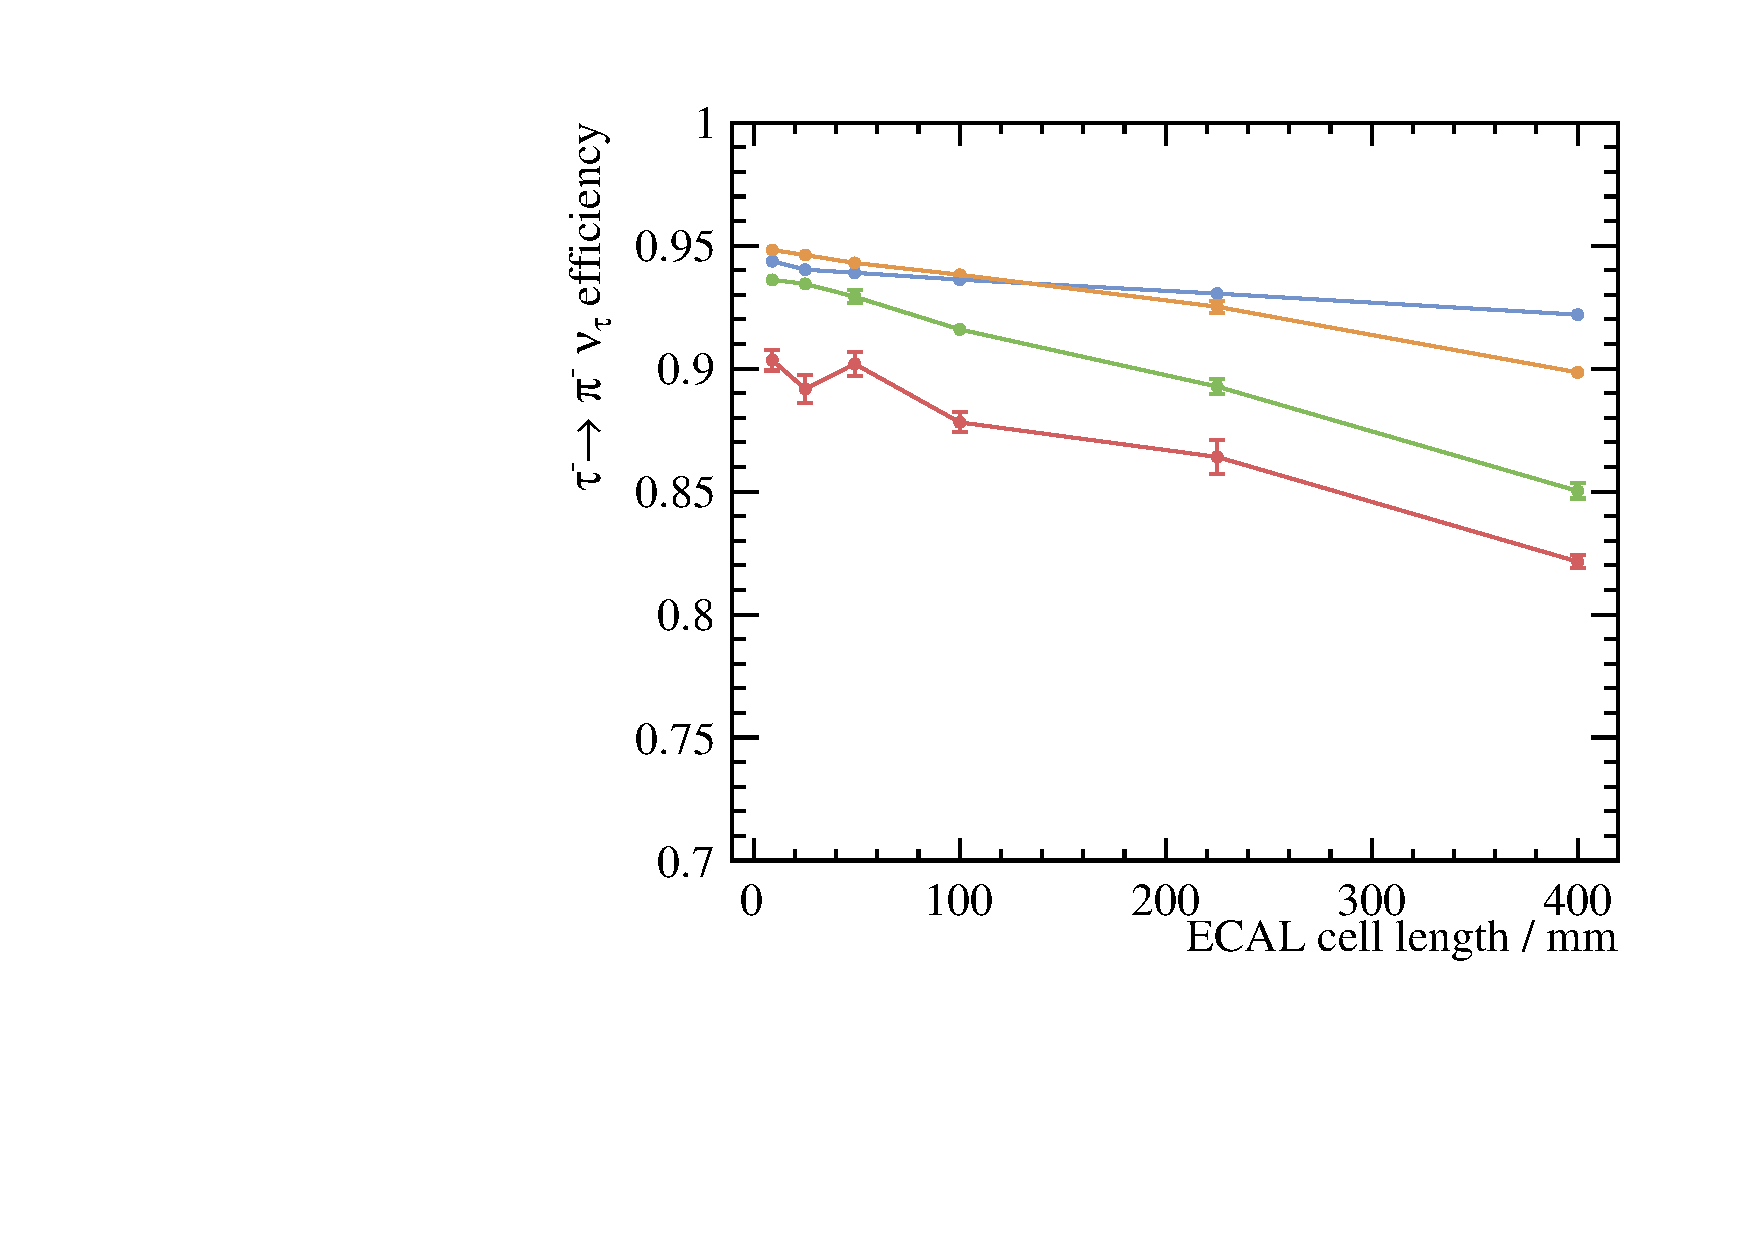
\includegraphics[width=\textwidth]{tau/plots3/decayMode2.pdf}
  \caption{}
  \label{fig:tauDecayMode2}
\end{subfigure}
\begin{subfigure}[b]{0.45\textwidth}
  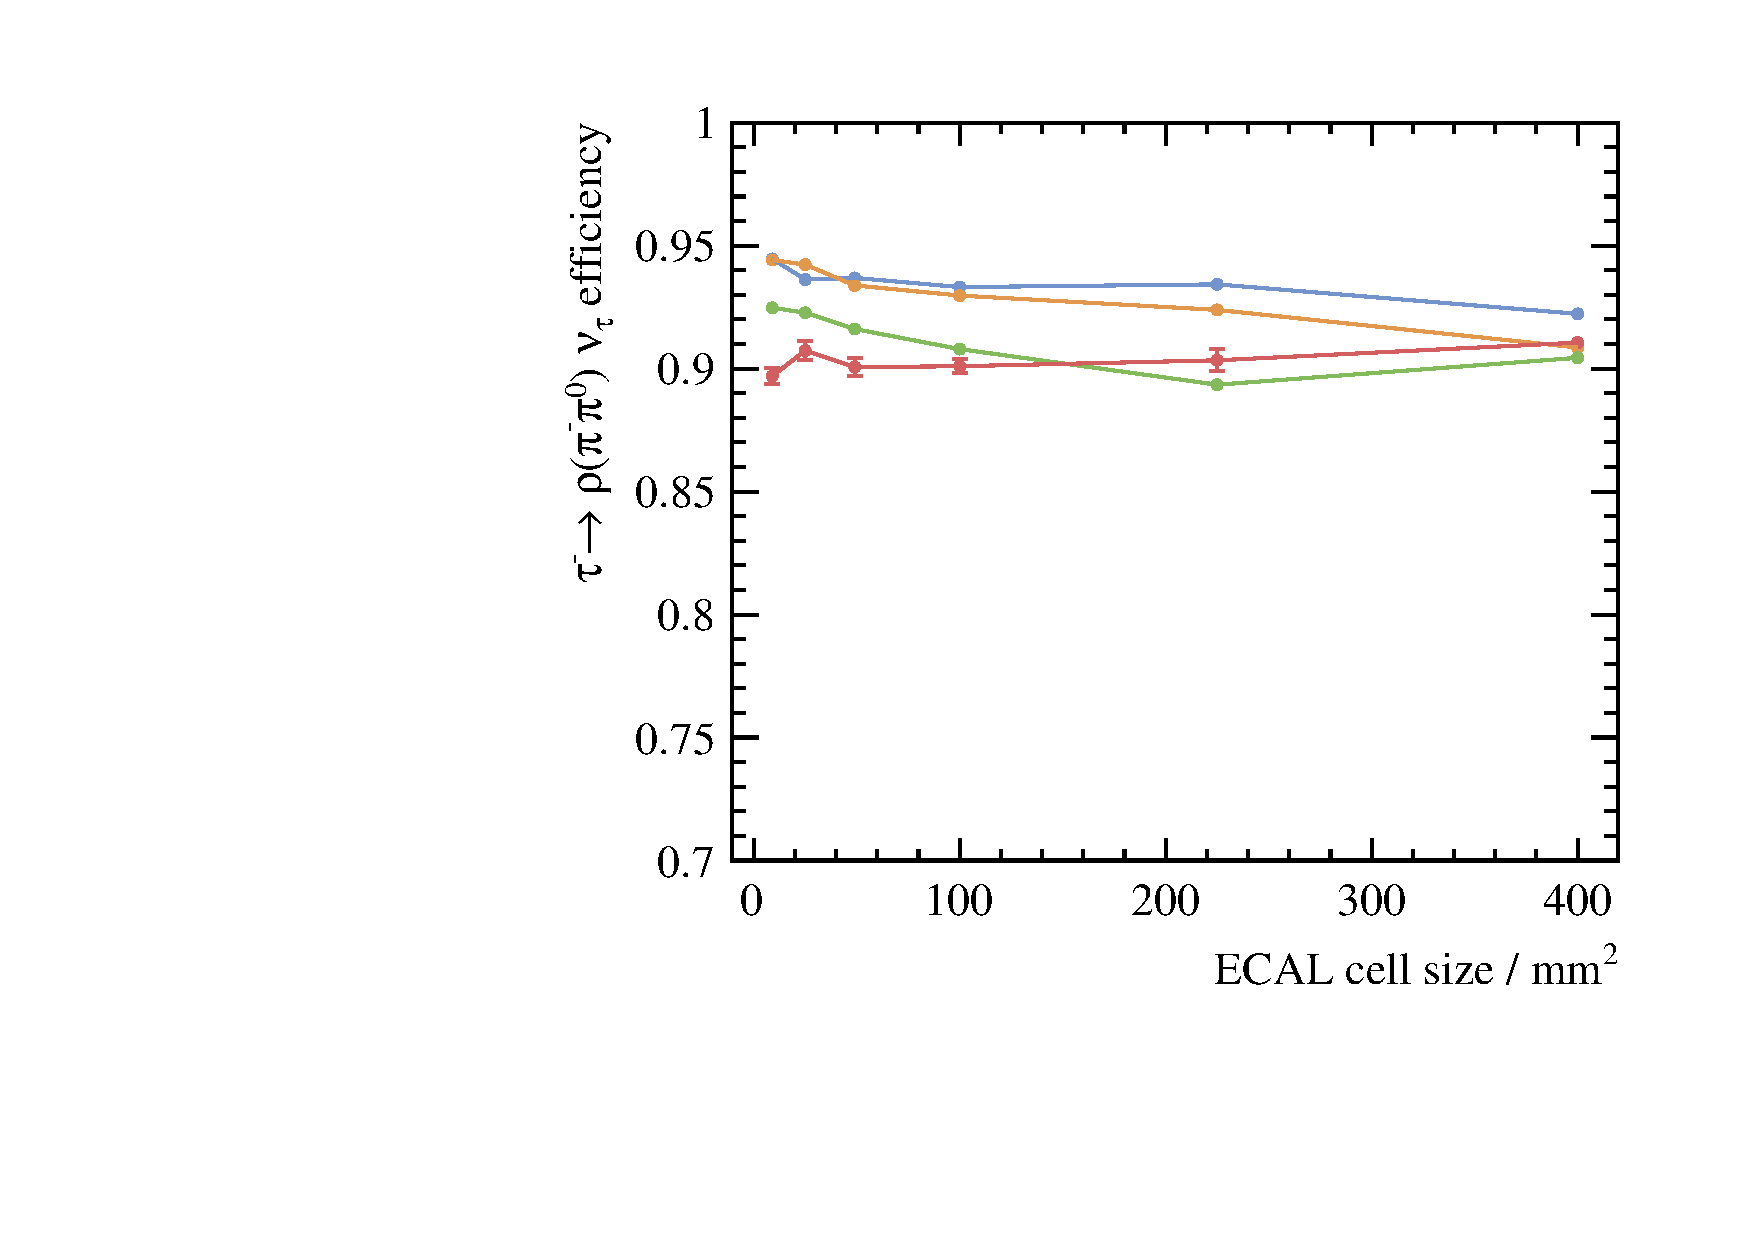
\includegraphics[width=\textwidth]{tau/plots3/decayMode3.pdf}
  \caption{}
  \label{fig:tauDecayMode3}
\end{subfigure}
\begin{subfigure}[b]{0.45\textwidth}
  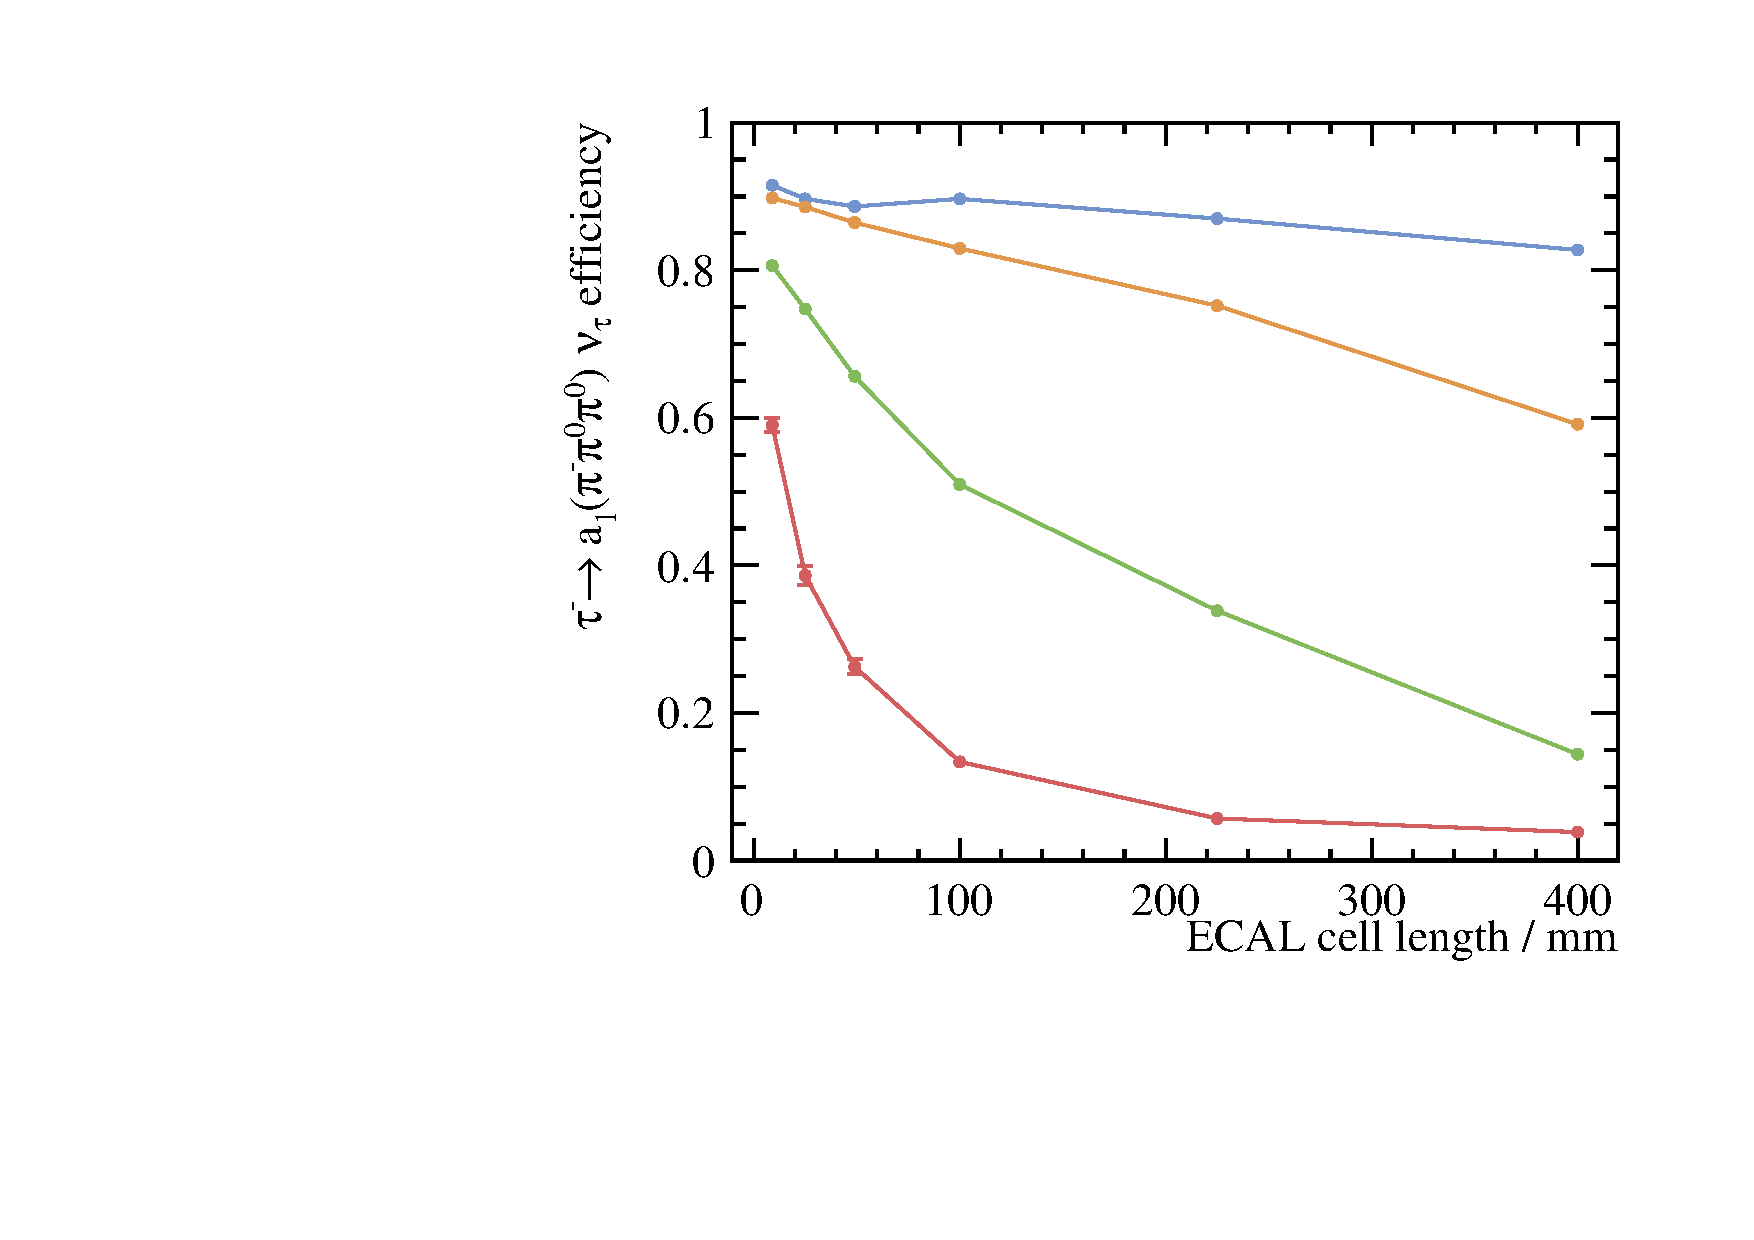
\includegraphics[width=\textwidth]{tau/plots3/decayMode4.pdf}
  \caption{}
  \label{fig:tauDecayMode4}
\end{subfigure}
\begin{subfigure}[b]{0.45\textwidth}
  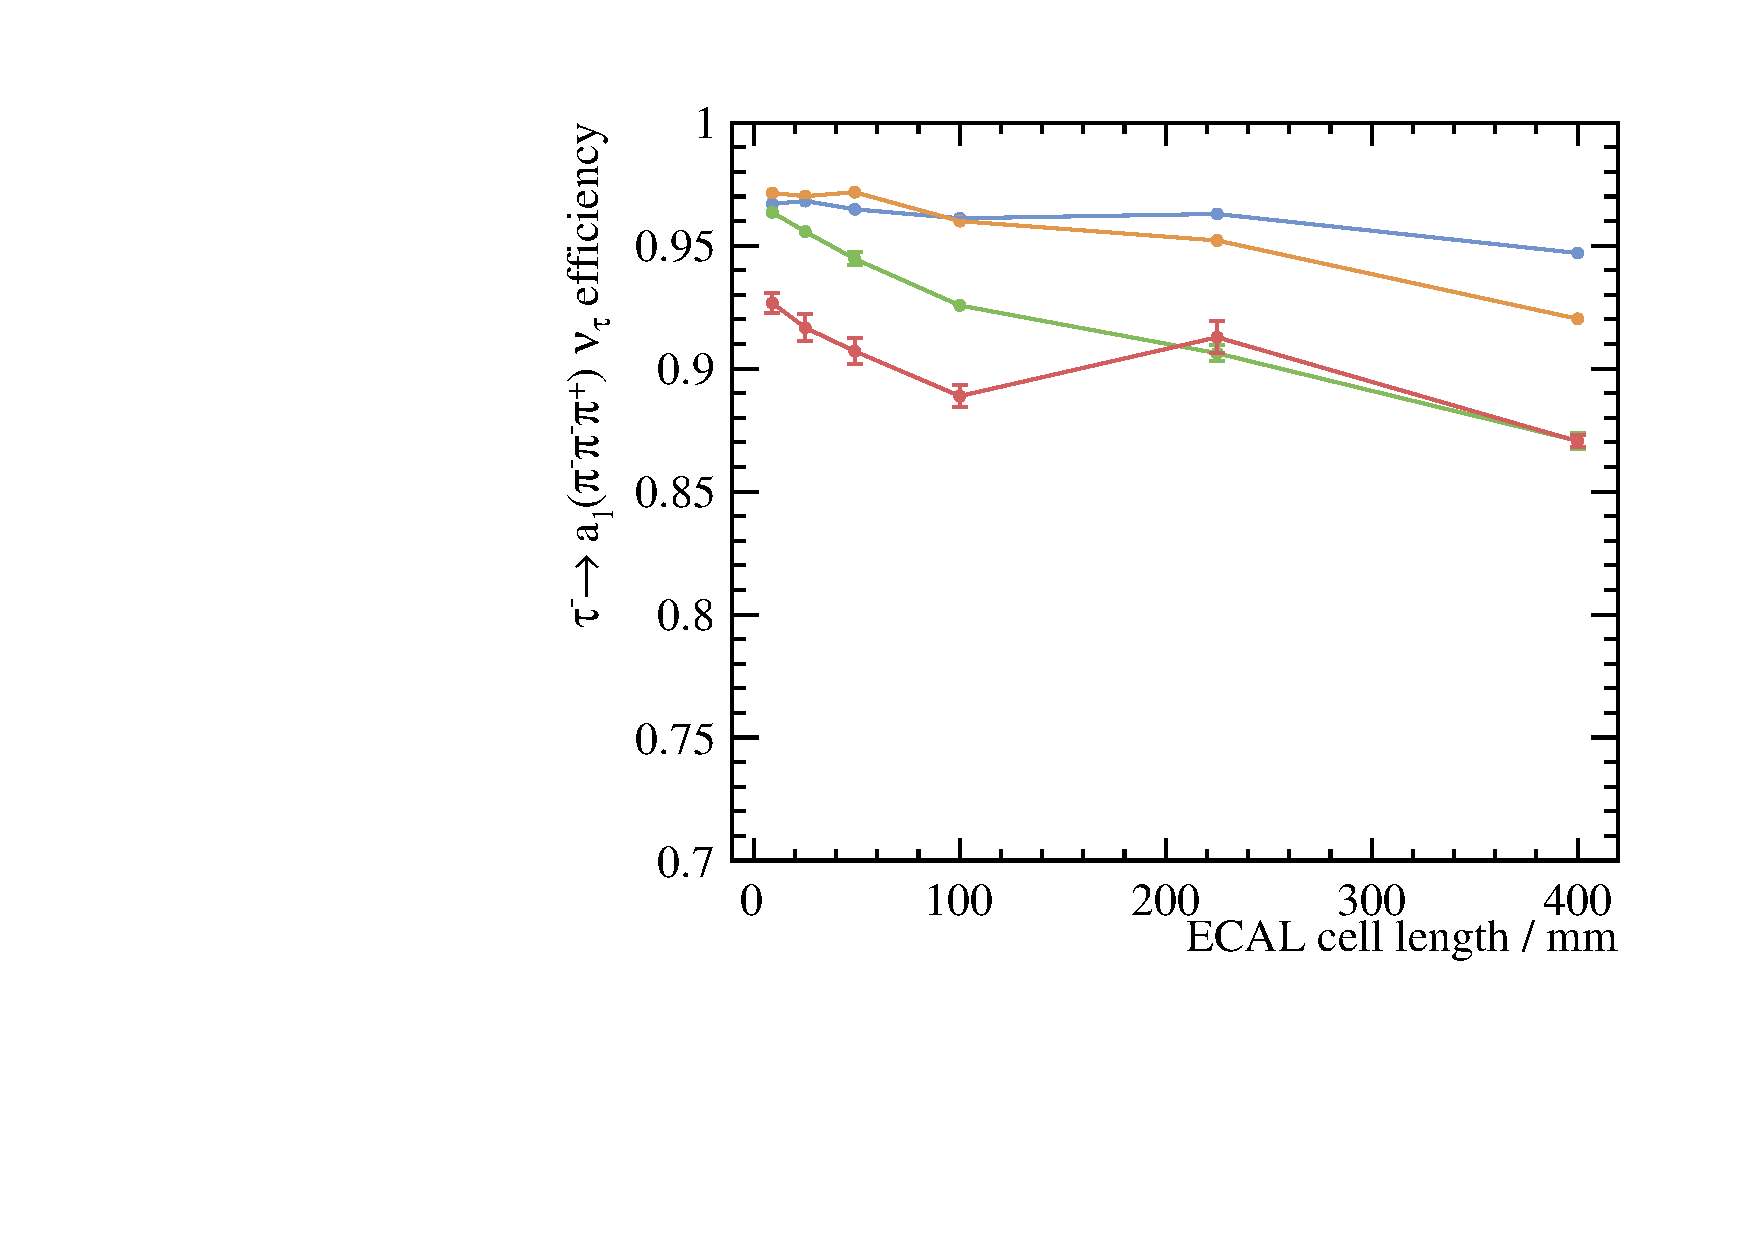
\includegraphics[width=\textwidth]{tau/plots3/decayMode5.pdf}
  \caption{}
  \label{fig:tauDecayMode5}
\end{subfigure}
\begin{subfigure}[b]{0.45\textwidth}
  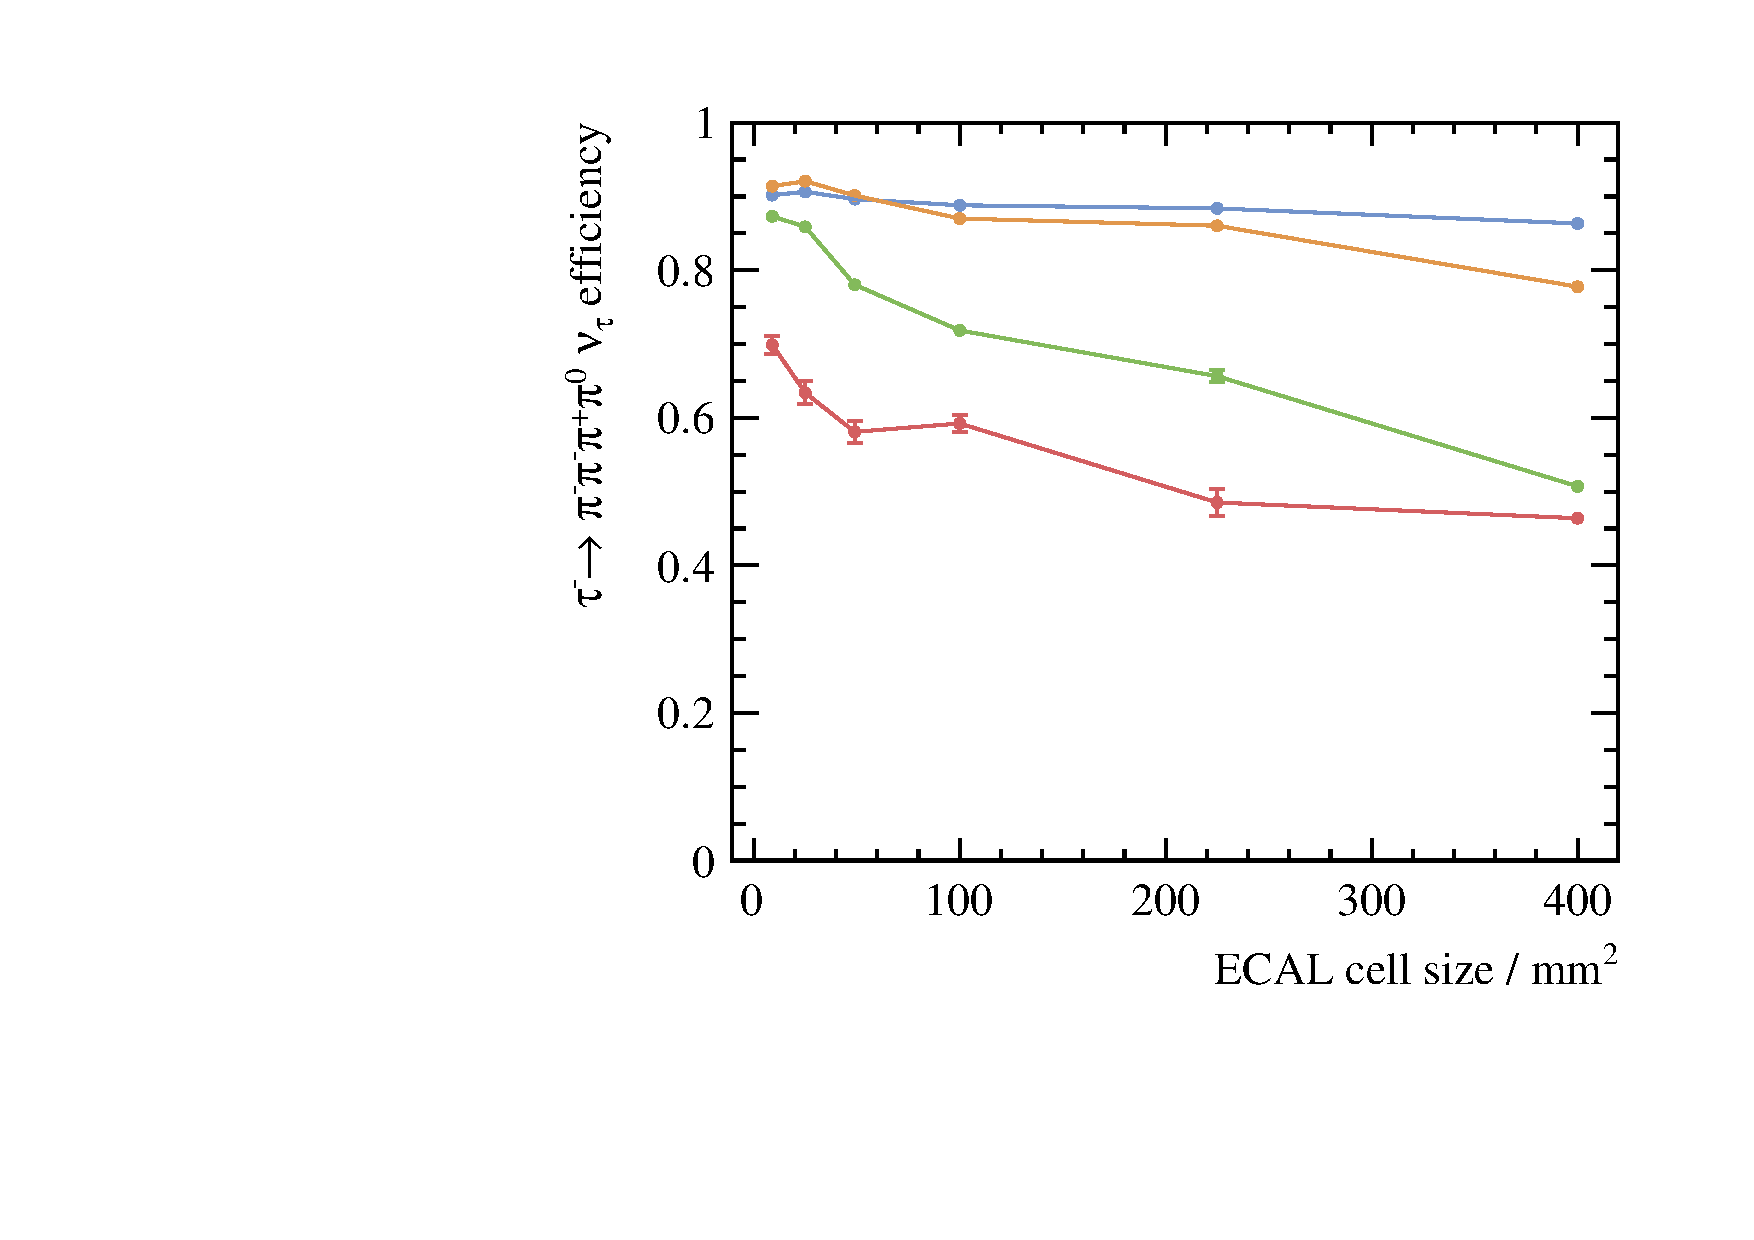
\includegraphics[width=\textwidth]{tau/plots3/decayMode6.pdf}
  \caption{}
  \label{fig:tauDecayMode6}
\end{subfigure}
\begin{subfigure}[b]{0.45\textwidth}
  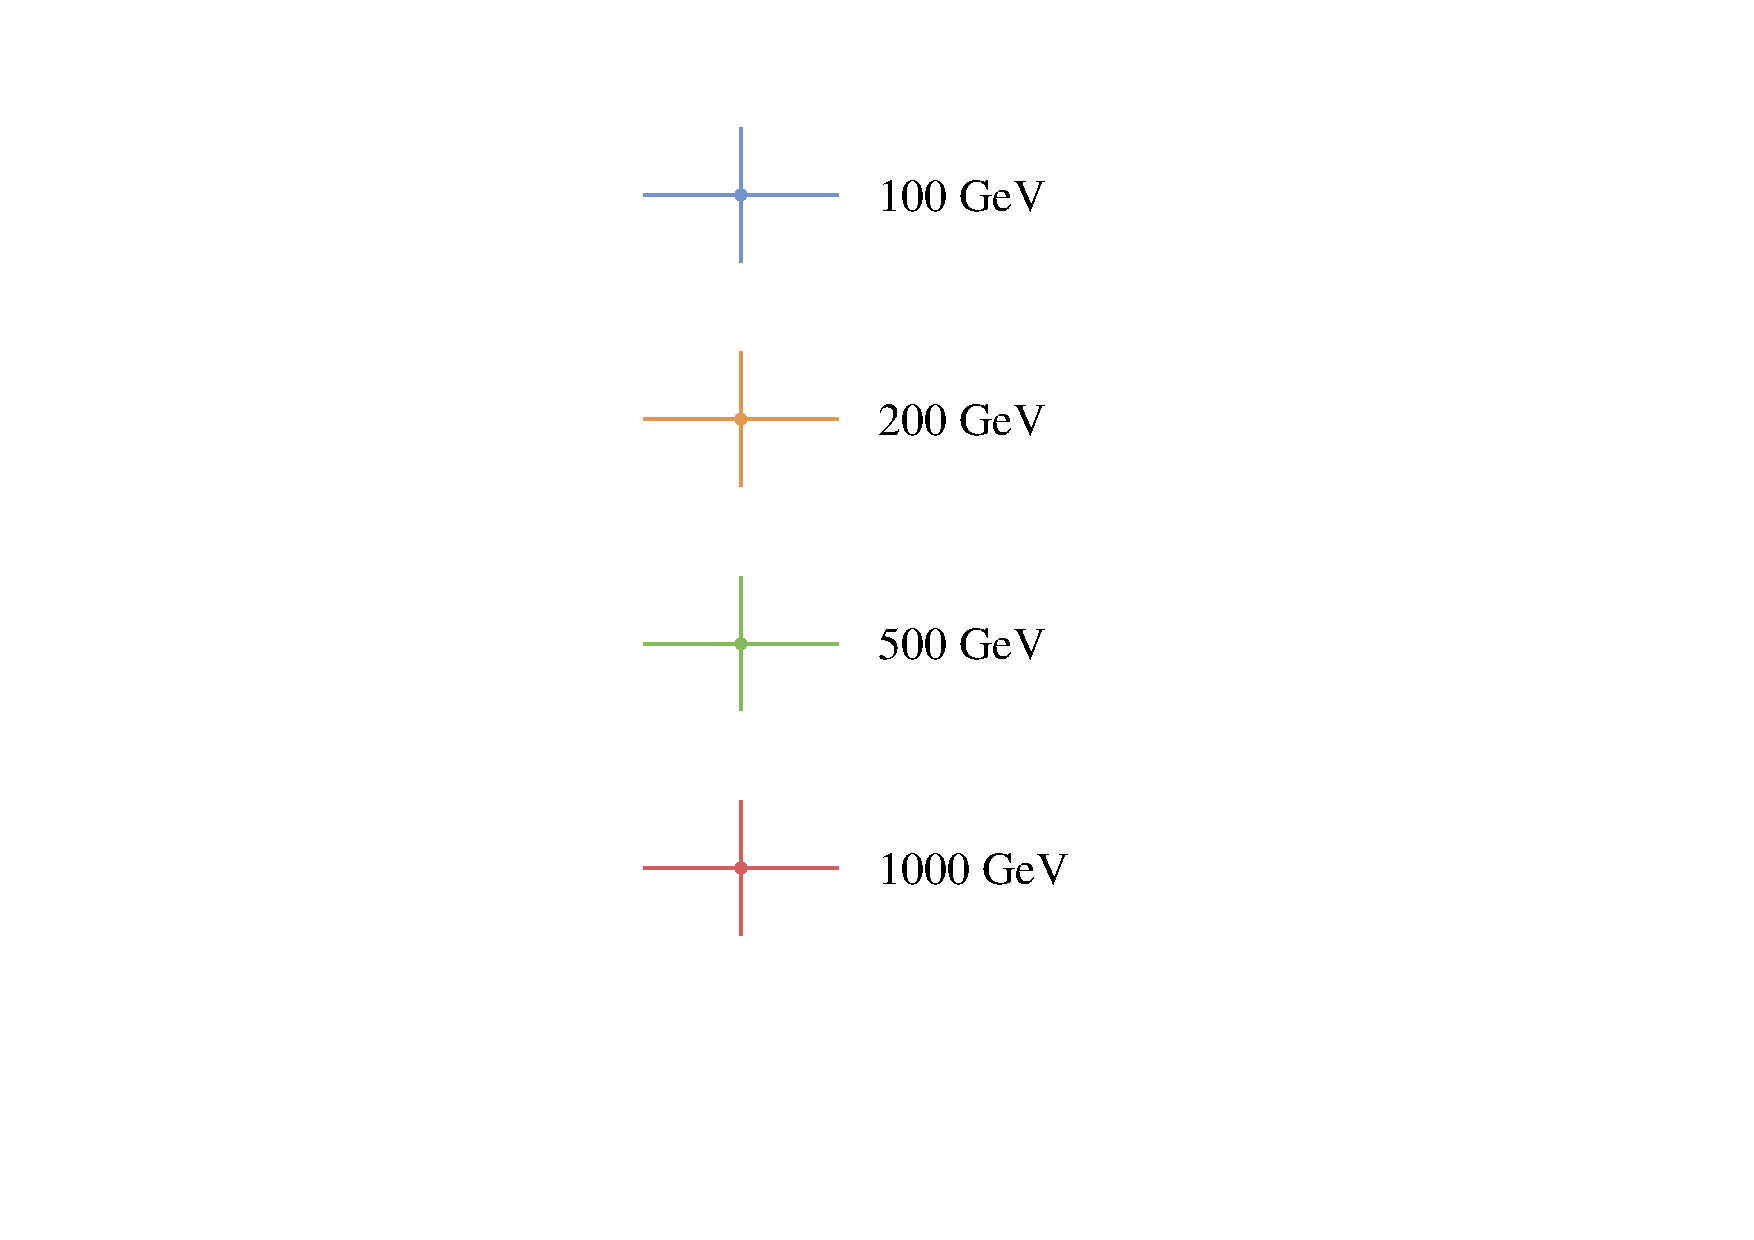
\includegraphics[width=\textwidth]{tau/plots3/legend.pdf}
  \caption{}
  \label{fig:tauDecayLegend}
\end{subfigure}
\caption[The correct classification efficiency for  tau hadronic decay final states  as a function of the \ECAL square cell sizes]
{ The correct classification efficiencies for  tau hadronic decay final states  as a function of the \ECAL square cell sizes for a) \decayPionShort decay mode, b) \decayRhoShortest decay mode, c) \decayAiPhotonShortest decay mode, d) \decayAiPionShortest decay mode, and e) \decayThreePionPhotonShort decay mode. The legend is shown in f). All plots are produced using  the \ILD detector model with \sqrtS = 100, 200, 500 and 1000\,GeV.}
\label{fig:TauPionEfficiency}
\end{figure}


\subsection{Tau hadronic decay correct classification efficiency}

There are two reasons to construct a single parameter for  overall tau decay efficiency: firstly the multivariate classifier is trained to optimised to achieve the best the overall classification efficiency; secondly it is easier to compare the impact of different detector models and different centre-of-mass energies with a single parameter.

The constructed tau hadronic decay correct classification efficiency, \tauHad, is a weighted correct classification efficiency for five hadronic decay modes:
\begin{equation}
\label{eq:had}
\tauHad = \frac{\sum_{i}^5 {Br}_{i}\varepsilon_{i}}{\sum_{i}^5 {Br}_{i}}  \,,
\end{equation}
where $Br_{i}$ is the branching fraction of the hadronic decay mode $i$  after the pre-selection cuts; $\varepsilon_{i}$ is the correct reconstruction efficiency of the decay mode $i$; and index $i$ is summed over five tau hadronic decay modes.

\FIGURE{fig:TauHadronicEfficiency} shows \tauHad as a function of \ECAL cell sizes with increasing centre-of-mass energies. The general trend for the \tauHad is that \tauHad decreases with the increase of centre-of-mass energies and the increase of \ECAL cell sizes, because it is increasingly difficult to reconstruct photons with boosted particles and lower \ECAL transverse spatial resolutions.

%As the \sqrtS increases, tau decay products are boosted and it is challenging to separate identical decay products. Similarly,  increasing \ECAL cell sizes makes particle separation more difficult.

At \rootSGeV{100}, the \tauHad decreases from 94\% at 3\,mm cell size, to 91\% at 20\,mm cell size. The decrease is approximately linear to the increase in the cell size. The decrease in \tauHad is greater at \rootSGeV{200}, where \tauHad declined from 94\% at 3\,mm cell size, to 86\% for a \ECAL cell size of  20\,mm. Most significant decrease in the \tauHad occurs at  \rootSGeV{500}, where the \tauHad decreases from 92\% at 3\,mm cell size, to 78\% at 20\,mm cell size. At \rootSGeV{1000}, the \tauHad drops from 85\% at 3\,mm cell size, to 75\% at 20\,mm cell size.

%From 10\,mm cell size onwards, the \tauHad decrease slows down.

The increase in \ECAL cell sizes has a larger impact on tau decay classification at high centre-of-mass energies. With decay products being spatially close at high centre-of-mass energies, it is more beneficial to have a smaller \ECAL cell size to reconstruct individual particle.

\begin{figure}[htbp]
\centering % \begin{center}/\end{center} takes some additional vertical space
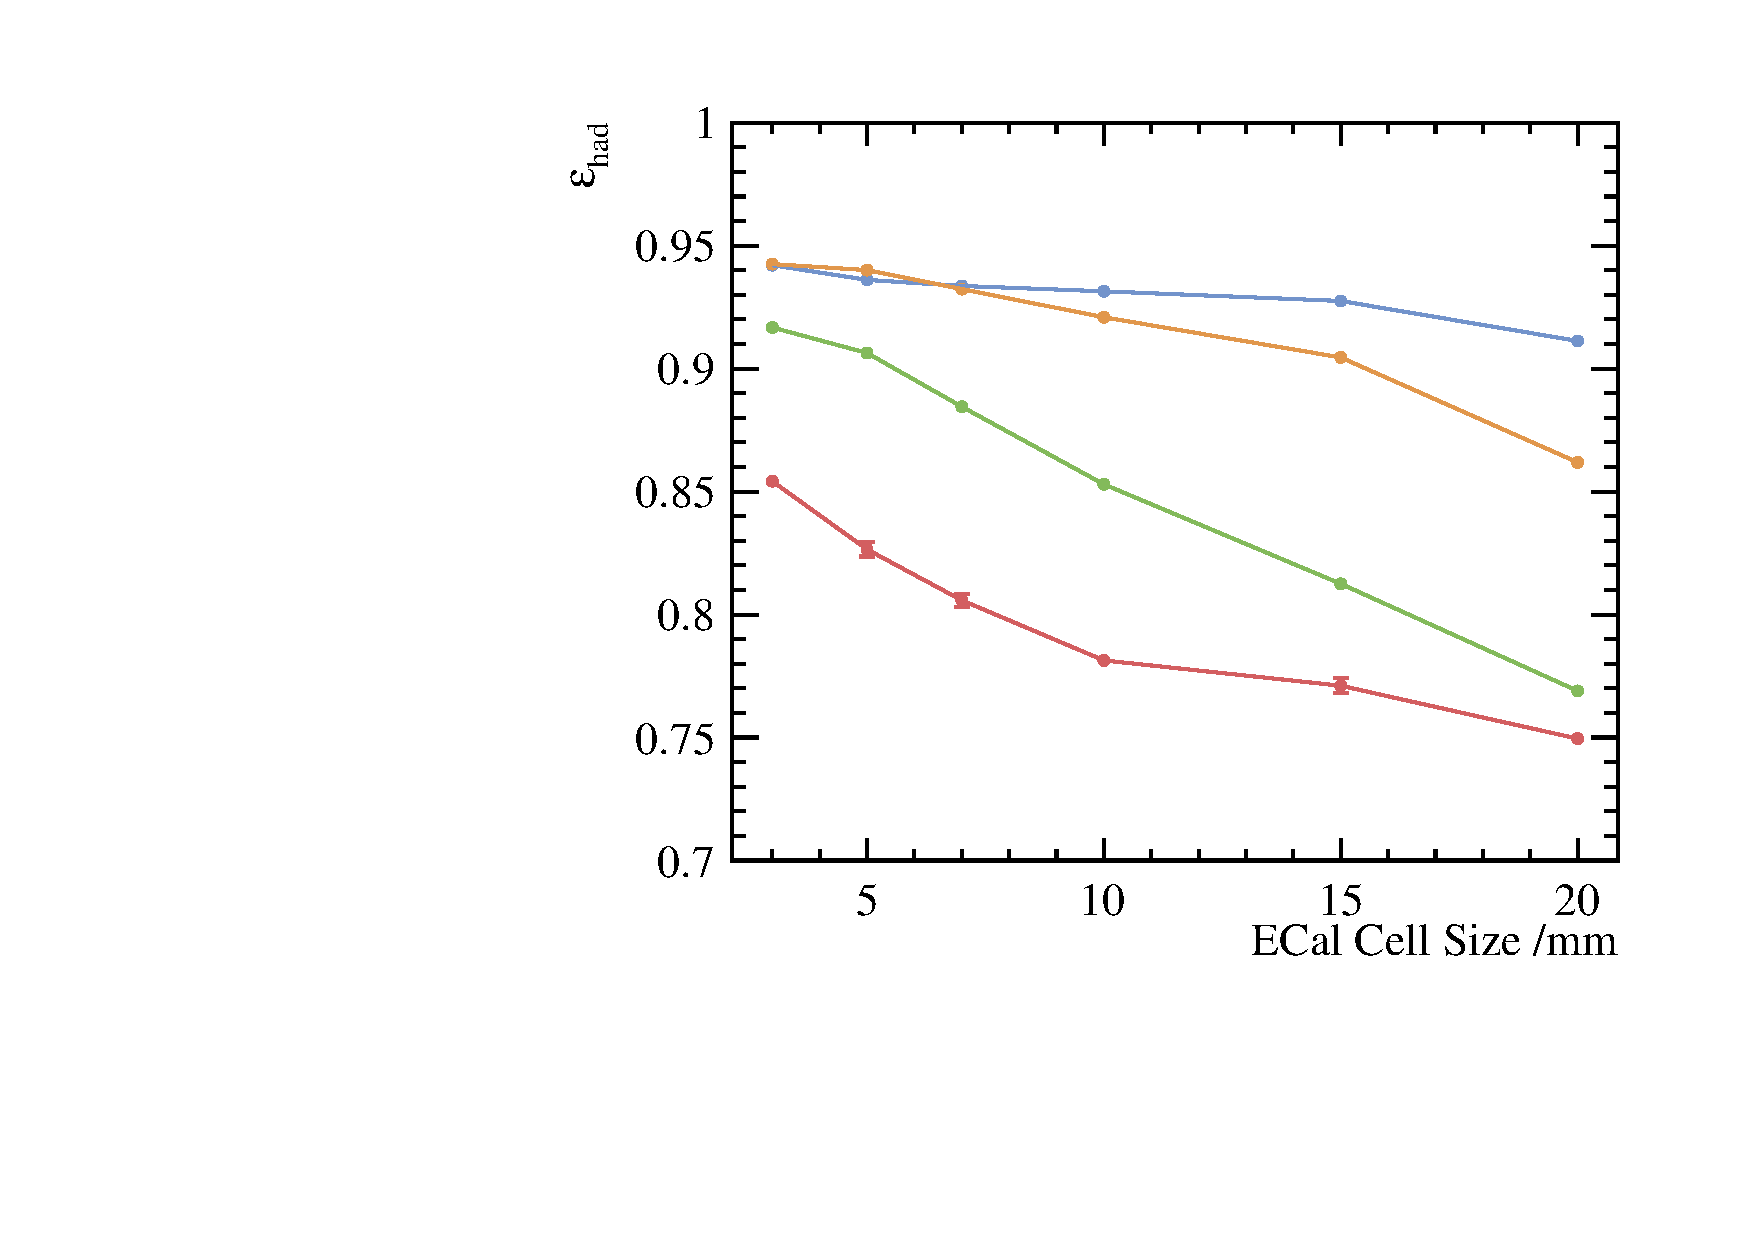
\includegraphics[width=.85\textwidth]{tau/plots3/hadronicEff.pdf}
\caption[The tau hadronic decay efficiency as a function of  the \ECAL cell sizes at different \sqrtS with the \ILD detector model.]
{The tau hadronic decay efficiency, \tauHad, as a function of  the \ECAL cell sizes with different centre-of-mass energies using the \ILD detector model. The blue, orange, green and red lines  represent the efficiencies at \sqrtS = 100, 200, 500 and 1000\,GeV respectively.}
\label{fig:TauHadronicEfficiency}
\end{figure}


\section{Tau pair polarisation correlations as a signature of Higgs boson}
\label{sec:tauHZ}

Many BSM theories predict the \HigssTauTau coupling would dominate the Higgs boson to leptons couplings  \cite{Duperrin:2008in}. Therefore, if an experiment observes an excess of tau pair decay events, it could be an indication of the Higgs boson. Here, this section follows the theoretical discussion in \Section{sec:theoryTauPair} to present a proof-of-principle analysis using tau pair polarisation correlation as a signature of Higgs boson.


Comparing \HiggsToTauTau  and \ZToTauTau, the difference in the spin of the bosons reflects in the different polarisation correlation of the tau pair. By extracting the polarisation correlations of the tau pair, the parent boson can be identified.

The subsequent sections discuss the ability to reconstruct the polarisation correlation of the tau pair with \ZToTauTau channel, where both \tauToPion. The analysis starts with the event pre-selection, followed by identifying the tau decay products in the events. Afterwards, the tau decay mode classification is used to identify \tauToPion decays. Lastly the tau pair polarisation correlation is presented and compared to the correlation distribution obtained with Monte Carlo simulation.

\subsection{Event pre-selection}

The channel to study is \HepProcess{\Pep \Pem \to \PZ \PZ}, where one \PZ decays hadronically and the other \PZ decays to a tau lepton pair. The samples were generated at \rootSGeV{350} without \ISR contribution for this proof-of-principle study.

The same seven tau decay modes in \Section{sec:tauDecayModes} are studied. The \tauToPion decay mode is selected for the proof-of-principle analysis of \PHiggs/\PZ separation with tau pair decay channel.

The event pre-selection is similar to that in \Section{sec:tauPreSel}. The cut on the total energy of non-neutrino decay products is not used, because a large fraction of \ZToTauTau events, where \tauToPion, has two low-energy charged pions. Therefore, the cut on the energy of non-neutrino decay products would throw away many events.


\subsection{Find tau decay products}
\label{sec:tauHZfindTau}
The final state of the selected channel, \eeZZQQ, contains two tau leptons and two quark jets. Therefore, tau decay products can either be found by direct tau lepton searching, or by using jet algorithms to find tau decay products as jets. If a tau lepton decays into a few particles, then the direct tau searching would work better. If a tau lepton decays into many particles, finding tau decay products as a jet has a better performance, as jet clustering works better with more particles. Hence, two approaches are combined to find the best tau pair.

\subsubsection{Direct tau searching}
Tau finder processer, \BonoTauFinder, is a modified version of the one in \Section{sec:doubleHiggsBonoTauFinder}. The basic idea is to find tau decay products consistent with tau decay topologies, and requires the tau  decay products to be isolated from the rest of the particles. Parameters chosen are set to find as many tau candidates as possible.

%The filtering of the candidates is via kinematic constraints.

\TABLE{tab:tauBonoTauFinderProcessor} lists all the cuts used in the \BonoTauFinder. Particles with transverse momentum (\pT) less than 0.5\,GeV are not considered. A seed particle is chosen and a search cone is formed around the seed, which requires one or three tracks with the invariant mass  of all particles inside the search cone less than 3\,GeV. The maximum search cone opening angle ($\theta_S$) is $\cos^{-1}(0.99)$. The isolation criteria states that the opening angle between the search cone  and the $2^{nd}$ closest track ($\theta_{cone,2^{nd}X^+}$) is larger than 0.6\,rad. If the criteria is satisfied,  the search cone with the tau seed is identified as a tau lepton.


\begin{table}[!htbp]
\begin{tabular}{lr}
\hline
\hline
Modified \BonoTauFinder  & Selection \\
\hline
Veto low \pT &  $\pT < 0.5$\,GeV\\
Seed particle & $\pT > 1$\,GeV \\
Maximum search cone opening angle  & $\theta_S \leqslant \cos^{-1}(0.99)$\\
Tau candidate rejection & $N_{X^+} \neq 1 \text{or} 3$; $m_{PFO} > 3$\,GeV   \\
Isolation & $\theta_{cone,2^{nd}X^+} > 0.6$\,rad\\
\hline
\hline
\end{tabular}
\caption
{Optimised parameters of the modified \BonoTauFinder.}
\label{tab:tauBonoTauFinderProcessor}
\end{table}

\subsubsection{Jet clustering}

Tau hadronically decay products can be also identified as a small jet. The Durham algorithm, also known as the \ee \kt algorithm, was used to form  jets (see \Section{sec:pandoraJetDurham}). The jet algorithm runs in the exclusive mode to find four jets for \eeZZQQ channel.

\subsubsection{Select tau candidates}

The best tau pair candidates are further selected using kinematic constraints. In  \HepProcess{\Pep \Pem \to \PZ \PZ} events, the energy of the \PZ is half of the centre-of-mass energy. The invariant mass of two quarks from \PZ should be close to \PZ mass. Therefore, the minimisation function utilising kinematic constraints is:
\begin{equation}
\chi^2 = \frac{\parenths{m_{\Pquark\Pquark} - m_{\PZ}}^2}{\sigma_{m_{\Pquark\Pquark}}^2} + \frac{\parenths{E_{\Pquark\Pquark} - \frac{\sqrtS}{2}}^2}{\sigma_{E_{\Pquark\Pquark}}^2},
\label{eq:tauMinimiser}
\end{equation}
where \sqrtS is the centre-of-mass energy; $m_{\PZ}$ is the mass of \PZ from reference \cite{Agashe:2014kda}; $\sigma_{m_{\Pquark\Pquark}}$ and $\sigma_{E_{\Pquark\Pquark}}$ are the reconstructed mass resolution  and energy resolution of the \ZToqq, respectively;  $m_{\Pquark\Pquark}$ and  $E_{\Pquark\Pquark}$ are defined differently for the direct tau searching and the jet clustering method; and the minimisation is iterated over all tau pairs from direct tau searching method or over all jets from jet clustering method. For the direct tau searching method, $m_{\Pquark\Pquark}$ and  $E_{\Pquark\Pquark}$ are obtained from the recoil momenta against two tau candidates, assuming collisions happening at \sqrtS: $m_{\Pquark\Pquark}$ is the invariant mass of the recoil momenta, and   $E_{\Pquark\Pquark}$ is the energy of the recoil momenta. For the jet clustering method,  $m_{\Pquark\Pquark}$ and  $E_{\Pquark\Pquark}$ are defined as the total invariant mass and energy of two jets.

The $\chi^2$ minimiser is repeated for the direct tau searching method and the jet clustering method. Each method selects a best tau pair candidate with the smallest $\chi^2$. Hence two tau pair candidates  are obtained. To find the best  overall tau pair candidate, a set of conditions is used. If the best tau pair candidate from both methods satisfies the kinematic constraint:
\begin{equation}
\absOf{m_{\Pquark\Pquark} - m_{\PZ}} < \sigma_{m_{\Pquark\Pquark}}\ , \absOf{E_{\Pquark\Pquark} - \frac{\sqrtS}{2}} < \sigma_{E_{\Pquark\Pquark}},
\label{eq:tauMinimiserSelector}
\end{equation}
the  tau pair candidate  with smallest $\chi^2$ is selected. Otherwise, if only one tau pair candidate satisfies the constraint in \Equation{eq:tauMinimiserSelector}, that candidate is chosen. If none of the candidates satisfies the constraint, and if one jet from the jet clustering is close to the beam pipe and there are exactly two tau candidates from \BonoTauFinder, then these two tau candidates are chosen. This is because if one jet is close to the beam pipe, it is likely that some particles close to the jet are undetected, which leads to a failure in the kinematic constraint or the jet reconstruction. Lastly, if all conditions above are not satisfied, two smallest jets by the number of \PFOs are chosen to be the best tau pair candidate.

\subsection{Boost tau decay products to \PZ decay rest frame}

The previous section describes the method to identify the tau pair decay products.  To use the tau decay mode classifier, it is necessary to know the tau lepton energy. For the channel \HepProcess{\PZ \to \APtauon \Ptauon}, the  energy of the tau lepton can only be obtained in \ZTauTau decay rest frame, which is half of the \PZ energy in the \ZTauTau rest frame. Hence the tau decay products need to be boosted to the \PZ decay rest frame for the calculation of the variables used in the MVA classification. The boosting requires the \fourMomentum of the \PZ.

The \fourMomentum of the \PZ decaying to tau pair is calculated from the recoil momenta of non tau-decay-products:
\begin{equation}
p^{\mu}_{\Ptau\Ptau} =
  \begin{pmatrix}
    \sqrtS\\   \sqrtS\times\sin\parenths{\theta_{beam}}\\  0   \\       0 \\
  \end{pmatrix}
  - \sum_{i}^{non-\Ptau}p^{\mu}_{i},
\end{equation}
where $\theta_{beam}$ is the beam crossing angle; \sqrtS is the centre-of-mass energy; $p^{\mu}_{i}$ is the four-momentum vector of the particle $i$; $p^{\mu}_{\Ptau\Ptau}$ is the four-momentum vector of the \PZ, where \ZToTauTau; and  index $i$ is summed over all non-tau-decay-product \PFOs. Extra kinematic constraint fixes the energy of the $p^{\mu}_{\Ptau\Ptau}$ to be half of \sqrtS:
\begin{equation}
p^{\mu}_{\Ptau\Ptau,correct} \equiv p^{\mu}_{\Ptau\Ptau} \times \frac{\frac{1}{2}\sqrtS}{E_{\Ptau\Ptau}},
\end{equation}
where $E_{\Ptau\Ptau}$ is the energy of the vector $p^{\mu}_{\Ptau\Ptau}$  and other variables are defined in the same way as in the previous equation. $p^{\mu}_{\Ptau\Ptau,correct} $ is then treated as the four-momentum vector of \PZ, where \ZToTauTau. Tau decay products are boosted to the \PZ decay rest frame accordingly. The calculation of the variables used in the MVA classifier are then performed in the \ZToqq decay rest frame.

\subsection{Variables used in the MVA}

Variables used in  the MVA classifier are a subset of the ones used in the previous analysis. Variables regarding EM shower profiles, calorimeter hit information and track information are not used (the last three rows in \Table{tab:tauVaraibles}) as the information was not available in the standard version of \pandora used in this analysis.

%Also for the computational reason, it was not feasible to use these variables for the MVA. \Pep and \Ppiplus separation could be improved if these extra variables are included.


\subsection{Multivariate analysis}

Half of the randomly selected sample is used to train the multivariate classifier,  which follows the procedure in  \Section{sec:tauMVA}. The same classifier as in the previous analysis  is used.   In the classifier applying stage, \tauToPion decay mode is selected with an additional criteria that there is at least one \Ppipm among the tau decay products.

\subsection{Result}

\FIGURE{fig:TauSpin2D} shows the two-dimensional plot of tau pair polarisation correlations from \PZ decay,  using \tauToPion decay mode, with \eeZZ channel where one \PZ decays to a tau pair and the other \PZ decays hadronically. The energy fractions of the tau decay product to the tau lepton are the appropriate kinematic variables, motivated in the theoretical discussion in \Section{sec:theoryTauPair}. \FIGURE{fig:TauSpin2DMC} shows the distribution obtained with the Monte Carlo particles. \FIGURE{fig:TauSpin2Dreco} shows the distribution using full detector simulation. Dark regions along the diagonal can be seen in both the distribution for the full detector simulation and the distribution for the Monte Carlo simulation. In the \ZToTauTau decays, an energetic \Ppiplus is likely to be associated with an energetic \Ppiminus and a low-energy \Ppiplus is  likely to be associated with a low-energy \Ppiminus. This trend is shown in both the distribution produced with the Monte Carlo particles and with the full detector simulation. Comparing the two figures in \FIGURE{fig:TauSpin2D}, some events in the top right quadrant, resembling both \Ppipm being energetic, are not reconstructed correctly. This is due to the incorrect finding of the tau pair decay products (\Section{sec:tauHZfindTau}).

This proof-of-principle analysis shows the tau polarisation correlations with \ZToTauTau decay where \tauToPion can be observed with \ILD detector model. With a similar study of \HiggsToTauTau,  the tau polarisation correlations can be used to separate Higgs boson from \PZ boson, and to identify Higgs boson in an experiment that observes the breaking of the lepton universality by favouring tau pair events.


\begin{figure}[htbp]
\centering % \begin{center}/\end{center} takes some additional vertical space
\begin{subfigure}[b]{0.75\textwidth}
  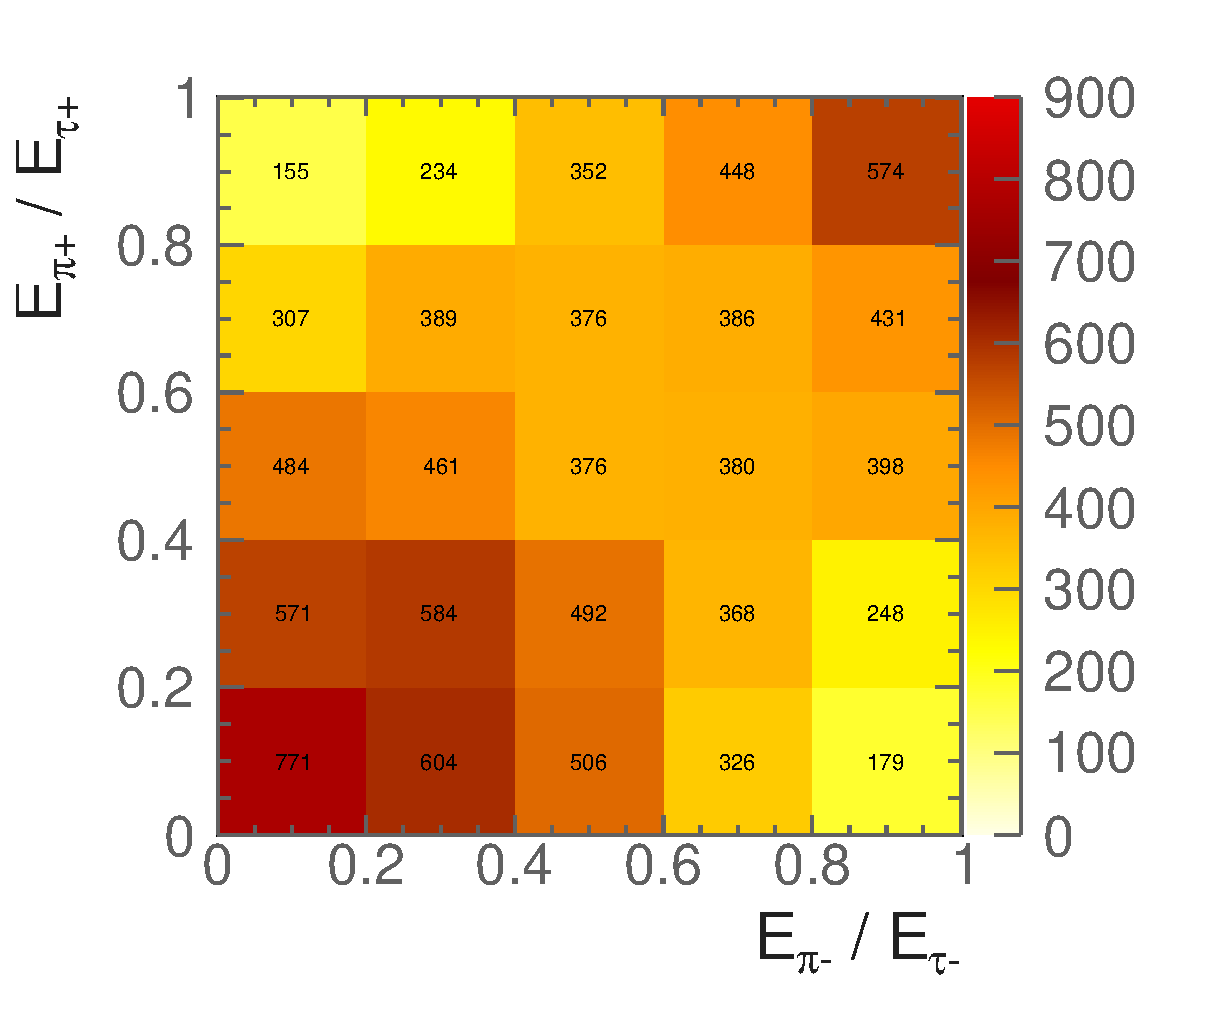
\includegraphics[width=\textwidth]{tau/NoTimeAnalysis/2DMC}
  \caption{Monte Carlo particles}
  \label{fig:TauSpin2DMC}
\end{subfigure}
\begin{subfigure}[b]{0.75\textwidth}
  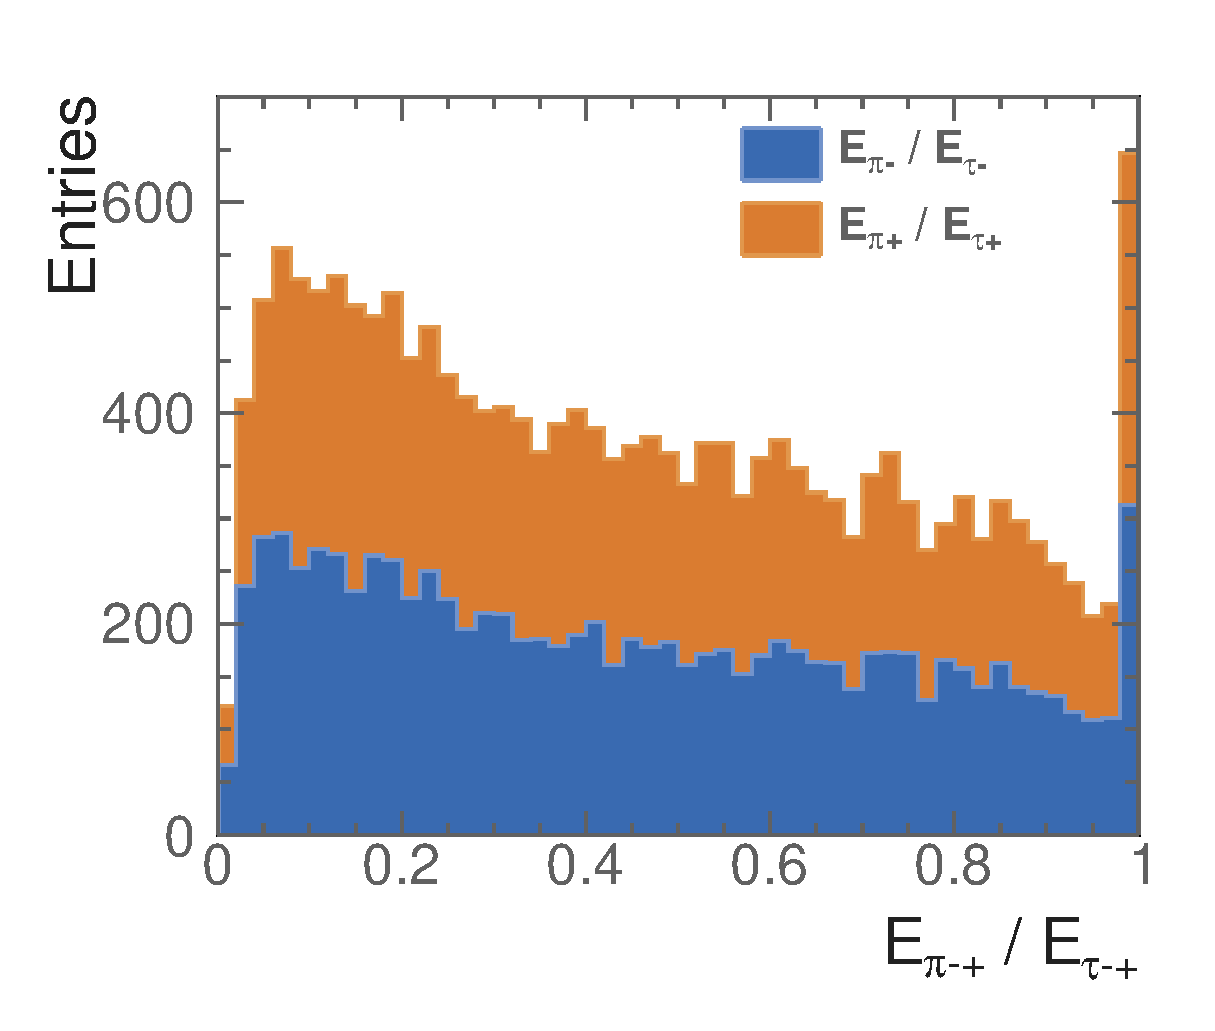
\includegraphics[width=\textwidth]{tau/NoTimeAnalysis/2Dreco}
  \caption{Simulated and reconstructed particles}
  \label{fig:TauSpin2Dreco}
\end{subfigure}
\caption
{Two-dimensional histograms of $E_{\Ppiplus}/E{\APtauon}$ as a function of $E_{\Ppiminus}/E{\Ptauon}$ obtained with  \ZToTauTau channel , selecting \tauToPion decay mode for both taus, for a) Monte Carlo particles, and b) simulated and reconstructed particles.}
\label{fig:TauSpin2D}
\end{figure}
\begin{comment}
\begin{figure}[htbp]
\centering % \begin{center}/\end{center} takes some additional vertical space
\begin{subfigure}[b]{0.45\textwidth}
  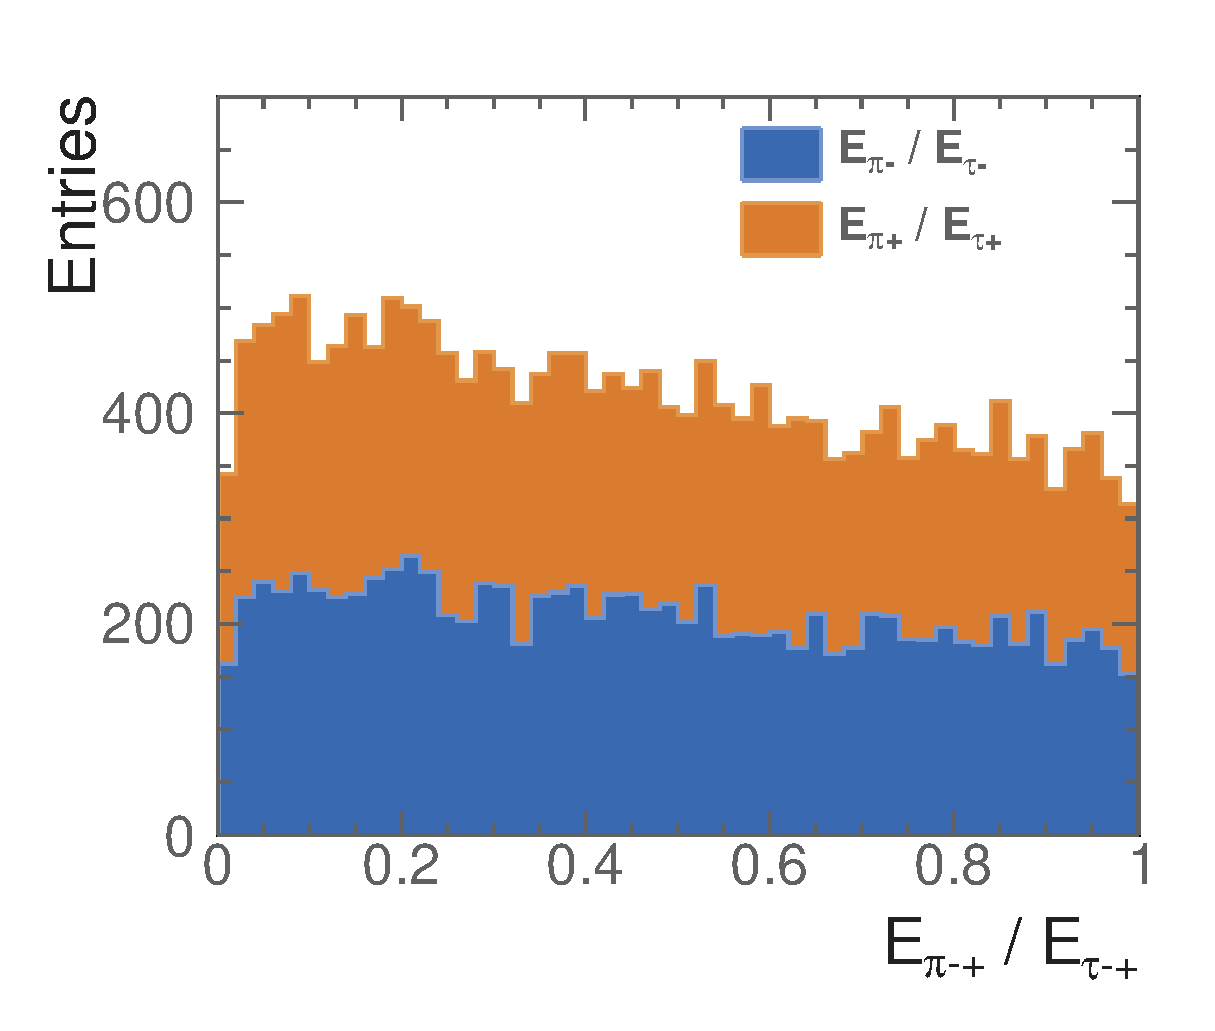
\includegraphics[width=\textwidth]{tau/NoTimeAnalysis/1DMC}
  \caption{Truth info.}
  \label{fig:TauSpin1DMC}
\end{subfigure}
\begin{subfigure}[b]{0.45\textwidth}
  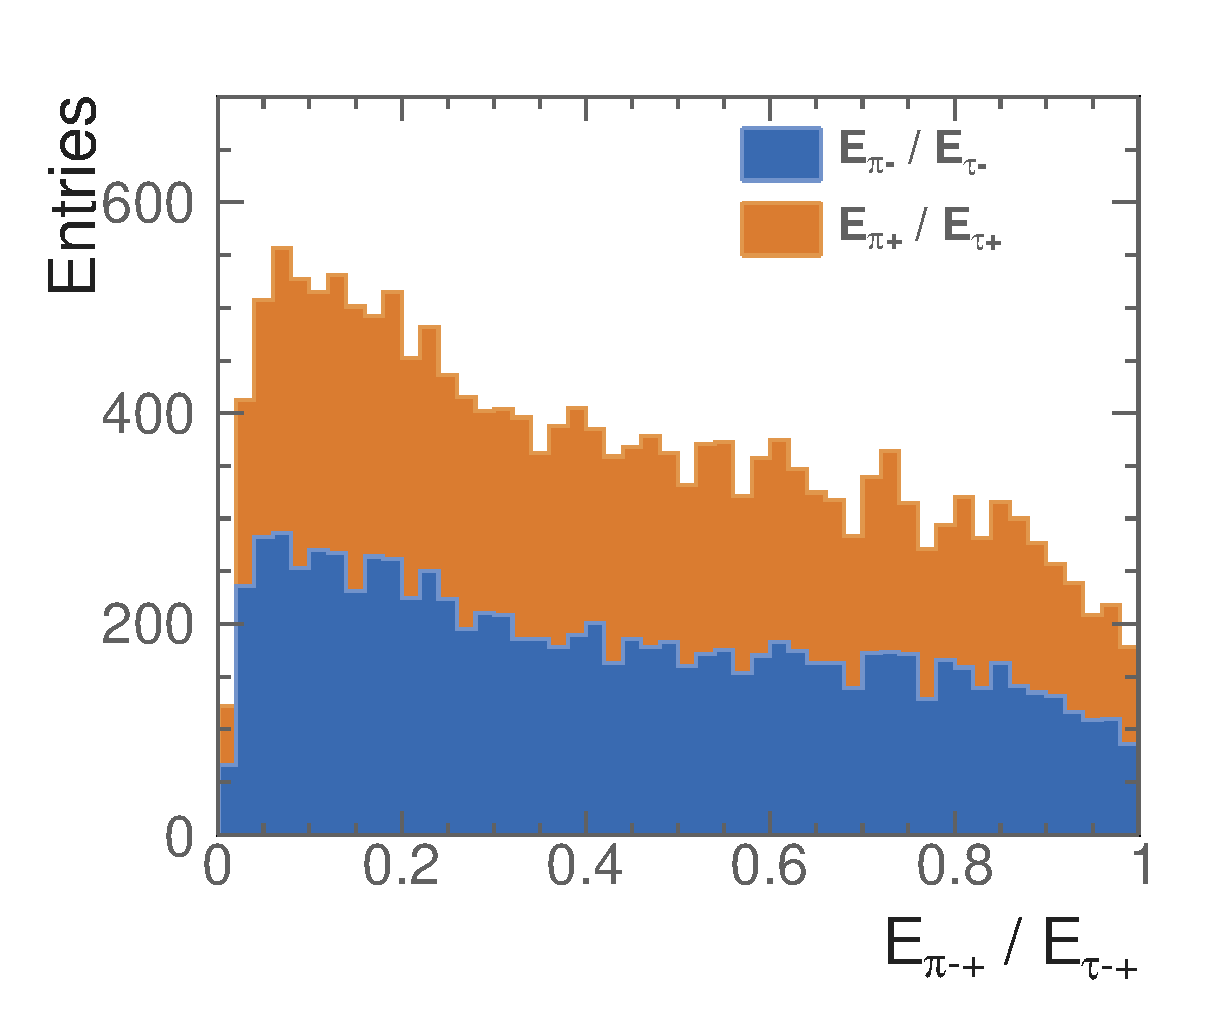
\includegraphics[width=\textwidth]{tau/NoTimeAnalysis/1DrecoNoOverflow}
  \caption{Reconstructed}
  \label{fig:TauSpin1Dreco}
\end{subfigure}
\caption[One-dimensional plot of spin correlations of the tau lepton pair from \PZ decay, using \decayPionShort decay mode.]
{One-dimensional plot of spin correlations of the tau lepton pair from \PZ decay, using \decayPionShort decay mode.}
\label{fig:TauSpin1D}
\end{figure}

\end{comment} 